\documentclass[a4paper,11pt]{article}%
    
\usepackage{fullpage}%
\usepackage[T1]{fontenc}%
\usepackage[utf8]{inputenc}%


\usepackage[french]{babel}% % Adjust the main language


\usepackage{graphicx}%
\usepackage{url}%
\usepackage{abstract}%
\usepackage{lipsum}
\usepackage{mathpazo}%
\usepackage{multicol}
\usepackage{listings}%
\usepackage[linesnumbered,ruled,vlined]{algorithm2e}
\usepackage{subcaption}
\usepackage{xcolor}
\usepackage{float} 

\parskip=0.5\baselineskip
\providecommand{\keywords}[1]{\textbf{\textit{Mots-clés : }} #1}
\sloppy

\begin{document}

\title{Création d'une \emph{Learning Heuristic} pour résoudre le \emph{Capacitated Vehicle Routing Problem}}

\author{Clément Legrand-Lixon}

\maketitle

\begin{abstract}
De nombreux algorithmes font régulièrement leur apparition pour tenter de résoudre des problèmes d'optimisation combinatoire, comme le \emph{Capacitated Vehicle Routing Problem}, ou d'améliorer des solutions existantes.
Dans la plupart des problèmes, il est possible d'extraire de la connaissance de petites instances résolues, afin de guider les algorithmes lors de la résolution de plus grandes instances. Intégrer de cette manière de la connaissance à un algorithme permet de créer une \emph{Learning Heuristic}, souvent plus performante que l'algorithme initial. 
\end{abstract}

\keywords{\emph{Optimisation combinatoire}, \emph{Capacitated Vehicle Routing Problem}, \emph{Extraction de connaissances}, \emph{Intégration de connaissances}, \emph{Learning Heuristic}}

\begin{description}
\item[Référence:] Stage effectué du 22 Mai 2018 au 27 Juillet 2018 au laboratoire CRIStAL à Lille sous la direction de Laetitia Jourdan, Univ Lille, CNRS - UMR 9189, F-59600 Lille, France.

\end{description}

\section*{Introduction}

Les problèmes d'optimisation combinatoire sont généralement des problèmes difficiles à résoudre~\cite{Papadimitriou_1982}, puisque le nombre de solutions à tester varie de manière exponentielle en la taille de l'instance. 
Le Vehicle Routing Problem (VRP) est un problème dit d'optimisation combinatoire.
L'objectif est de relier un nombre $n$ de clients par des véhicules, démarrant et finissant tous à un même point défini, le dépôt. 
Ce problème est NP-complet, et dispose de nombreuses variantes (ajout d'une contrainte de temps, plusieurs dépôts possibles...). Cela permet de modéliser un grand nombre de situations réelles. 
L'une des variantes les plus connues consiste à prendre en compte pour chaque client sa demande, de sorte à ce que les tournées créées ne dépassent pas une certaine capacité définie à l'avance, correspondant à la capacité du véhicule de transport. 
On nomme ce problème Capacitated Vehicle Routing Problem (CVRP). 

De nombreux types d'algorithme existent pour résoudre ces problèmes d'optimisation (algorithme génétique, colonie de fourmis...), comme le montre~\cite{synthese} dans le cas du CVRP, mais ne parviennent pas toujours à trouver la solution optimale. 
De nombreuses heuristiques ont également vu le jour pour résoudre le CVRP, aucune d'entre elles ne parvient à trouver des solutions optimales pour toutes les instances de la littérature, malgré de très bons résultats dans la plupart des cas. Encore récemment~\cite{Sorensen_2017}, une nouvelle heuristique efficace a vu le jour. 
L'une des méthodes pour améliorer les algorithmes d'optimisation consiste en l'extraction de connaissances sur des petites instances résolues, puis leur intégration dans l'algorithme d'optimisation choisi.

La section~\ref{presentation} commence par présenter le problème étudié, et introduit les notations et opérateurs utilisés dans la suite. L'objectif fixé et la méthode mise en place pour y parvenir y sont également présentés.
La section~\ref{SolInit} explique comment obtenir une solution initiale au problème de bonne qualité, puis la section~\ref{opti} propose un algorithme d'optimisation utilisé pour la résolution du problème. 
La section~\ref{extraction} décrit comment  extraire de la connaissance des instances étudiées. 
Enfin, la section~\ref{Integration} explique comment intégrer de la connaissance à un algorithme d'optimisation et présente une nouvelle \emph{learning heuristic} pour résoudre le problème. 

\section{Présentation des notions et notations}
\label{presentation}
Cette section introduit dans un premier temps le problème étudié, en rappelant au préalable ce qu'est un problème d'optimisation combinatoire. Les différentes notations utilisées dans la suite du papier sont ensuite décrites, enfin l'objectif de cet article est présenté. 


\subsection{Description du problème}
De nombreux problèmes sont dits d'optimisation combinatoire, dont font notamment partie le \emph{Traveller Salesman Problem} (TSP), ainsi que le \emph{Capacitated Vehicle Problem} (CVRP). Cette partie détaille de manière formelle ce qu'est un problème d'optimisation combinatoire, puis présente le problème étudié : \emph{CVRP}

\subsubsection{Optimisation combinatoire}
Un problème d'optimisation combinatoire (également appelée optimisation discrète), consiste à trouver dans un ensemble discret, les meilleures solutions (au sens d'une certaine fonction, dite \emph{fonction objectif}) réalisables. 
Formellement, on a :

\begin{itemize}
\item Un ensemble discret $N$ de solutions;
\item Une fonction $f : 2^N \rightarrow \Re$, dite fonction objectif;
\item Un ensemble $R \subseteq N$, dont les éléments sont appelés solutions réalisables.
\end{itemize}

Ainsi, un problème d'optimisation combinatoire consiste à déterminer :

\begin{center}
$ min_{S \subseteq N} \{ f(S), S \in R \} $
\end{center}

Toutefois dans ce type de problème, le nombre de solutions réalisables varie généralement de manière exponentielle selon la taille du problème. Cela rend donc impossible une énumération complète des solutions réalisables, d'où la difficulté de trouver la solution optimale à ce type de problème.

\subsubsection{Vehicle Routing Problem (VRP)}

Le problème de tournées de véhicules, est un problème NP-complet d'optimisation combinatoire, où sont donnés $n$ points de coordonnées $(x_i,y_i)$, représentant 1 dépôt et $n-1$ clients. On dispose également d'une flotte de $k$ véhicules. 
L'objectif est de minimiser la longueur du réseau (i.e. l'ensemble des tournées effectuées par les véhicules, une \emph{tournée} correspondant à l'ensemble des clients desservis par un véhicule). 
En reprenant les notations de~\cite{cvrp_pres}, on définit $x_{i,j}^v$ qui vaut 1 si $j$ est desservi après $i$ par le véhicule $v$, et 0 sinon. 
On définit également $c_{i,j}$ comme étant la distance entre $i$ et $j$.
Ainsi une solution \emph{Sol} du problème est la donnée d'une matrice, telle que $Sol[i][j] = c_{i,j} x_{i,j}^v$.
On cherche donc à déterminer:
\begin{center}
$ min \sum_{i = 0}^{n} \sum_{j = 0}^{n} \sum_{v = 1}^{k} c_{i,j} x_{i,j}^v = min_{Sol}cost(Sol)$
\end{center}
La fonction $cost$ correspond à la fonction objectif de ce problème.

Les tournées créées doivent également respecter les contraintes suivantes :

\begin{itemize}
\item Chaque client doit être desservi par une et une seule tournée : $\forall i > 0 \sum_{j = 1}^{n} \sum_{v = 1}^{k} x_{i,j}^v = 1$;
\item Chaque tournée doit partir et s'arrêter au dépôt : $\forall v \sum_{j = 1}^{n} x_{0,j}^v = 1$ et $\sum_{j = 1}^{n} x_{j,0}^v = 1 $.
\end{itemize}

Un exemple d'instance est présenté en figure~\ref{Instance3205}, où les points rouges représentent les clients et le point bleu le dépôt. Une solution possible au problème est représenté en figure~\ref{SNC3205} mais n'est à priori pas optimale. 
De nombreux algorithmes ont vu le jour pour tenter de résoudre ce problème, ainsi que les nombreuses variantes qui existent (ajout de contraintes de capacité, temps ou longueur sur les tournées, ces contraintes sont cumulables). 
C'est l'ajout de capacité aux tournées qui nous intéressera plus particulièrement.



\begin{figure}
    \begin{minipage}[c]{.46\linewidth}
        \centering
		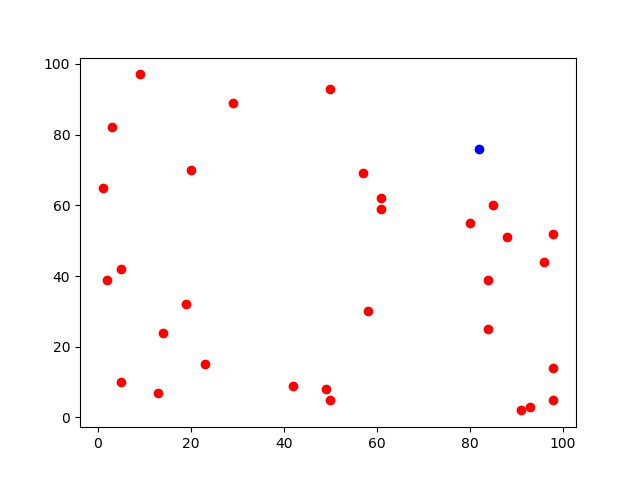
\includegraphics[scale=0.5]{Instance.png}
		\caption{Représentation de l'instance A-n32-k05 de la littérature (31 clients et 1 dépôt).}
		\label{Instance3205}
    \end{minipage}
    \hfill%
    \begin{minipage}[c]{.46\linewidth}
        \centering
        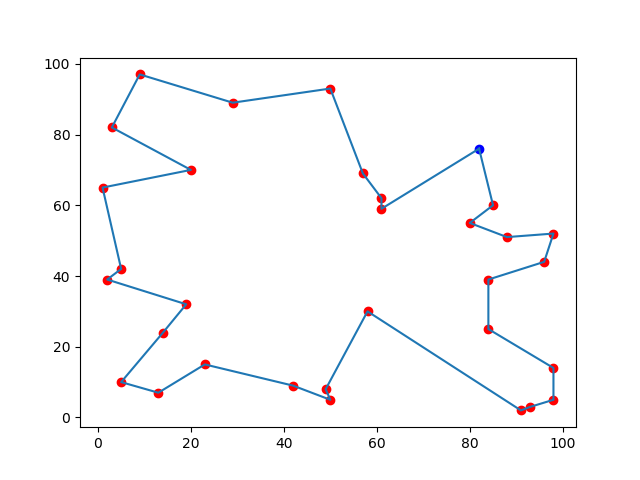
\includegraphics[scale=0.5]{solutionNoCapacity.png}
		\caption{Représentation d'une solution de l'instance A-n32-k05.}
		\label{SNC3205}
    \end{minipage}
\end{figure}

\subsubsection{Capacitated VRP (CVRP)}

On étend le VRP au CVRP en ajoutant à chaque client $i$ une demande $d_i$, ainsi qu'une capacité $C$ aux véhicules.
Une nouvelle contrainte vient donc s'ajouter aux contraintes classiques du VRP :

\begin{itemize}
\item La demande totale sur chaque tournée ne doit pas excéder la capacité du véhicule : $\forall v \sum_{i = 0}^{n} \sum_{j = 0}^{n} x_{i,j}^v d_j < C$.
\end{itemize}

Si on reprend l'instance A-n32-k05, en considérant les demandes des clients ainsi que la capacité disponible pour chaque véhicule, on obtient une solution présente sur la figure~\ref{SC3205}, qui n'est pas optimale. 
Ce problème est beaucoup étudié car il a de nombreuses applications (comme par exemple la gestion du trafic routier, ou alors la gestion d'un réseau de bus), et peu de solutions optimales ont été trouvées pour des instances de plus de $500$ clients. 

Les instances du CVRP étudiées par la suite, sont disponibles sur~\cite{cvrplib} 

\begin{figure}
\centering
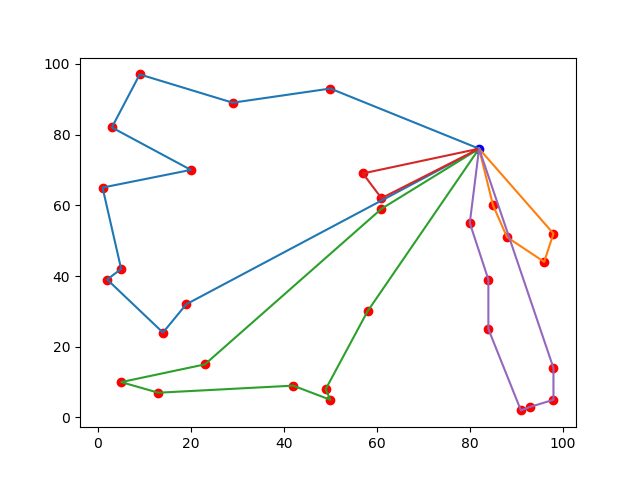
\includegraphics[scale=0.5]{solutionCapacity.png}
\caption{Représentation d'une solution de l'instance A-n32-k05, où les demandes des clients sont prises en compte. Elle comporte 5 tournées.}
\label{SC3205}
\end{figure}

\subsubsection{Méthodes de résolution de CVRP}
L'article~\cite{synthese} présente les différents types d'algorithme et méthodes qui existent pour résoudre le CVRP (et plus généralement un problème d'optimisation combinatoire).
Il distingue principalement deux types de méthodes : les méthodes exactes et les méthodes approchées.

Les méthodes exactes, ou encore méthodes \emph{complètes}, permettent de trouver la solution optimale au problème. 
Ces méthodes sont basées sur des explorations exhaustives de l'ensemble des solutions réalisables. 
Toutefois ces méthodes basiques restent inappropriées aux problèmes d'optimisation combinatoire. 
Il existe néanmoins des algorithmes qui permettent de restreindre l'ensemble à explorer en éliminant des sous-ensembles de mauvaises solutions à l'aide de techniques, dites d'élagage.

Contrairement aux méthodes exactes, les méthodes approchées sont dites \emph{incomplètes}, car elles permettent de trouver de bonnes solutions, mais ne garantissent pas l'optimalité de celles-ci. 
Cette méthode regroupe notamment les heuristiques et méta-heuristiques.

\textbf{Une heuristique} est un moyen de guider les choix que doit faire un algorithme pour réduire sa complexité. Une heuristique est spécifique à un problème et ne peut donc pas être généralisée.

\textbf{Une méta-heuristique} peut être considérée comme une heuristique "puissante et évoluée", dans la mesure où elle est généralisable à plusieurs problèmes d'optimisation. On classe souvent les méta-heuristiques en fonction du nombre de solutions qu'elles manipulent. Celles à solution unique (recherche tabou, descente du gradient), et celles à population de solutions (algorithmes génétiques et colonies de fourmis).

De plus les méthodes approchées doivent trouver un équilibre entre deux tendances opposées : l' \emph{intensification} (ou \emph{exploitation}) et la \emph{diversification} (ou \emph{exploration}). \textbf{L'intensification} de la recherche signifie que celle-ci se concentre autour des meilleures solutions rencontrées, considérées prometteuses. 
Alors que \textbf{la diversification} incite davantage la recherche à explorer des nouvelles zones de l'espace de solutions. 

Ainsi les méta-heuristiques à solution unique ont plus tendance à l'exploitation du voisinage de la solution en question, et les approches à base de population de
solutions ont plutôt tendance à l'exploration.



\subsection{Parcours et exploration des voisinages}
\label{voisinage}

Il existe plusieurs moyens pour procéder à une diversification de la solution courante~\cite{ME_2012}.
En effet, il est possible qu'en modifiant légèrement la solution courante, on obtienne une autre solution réalisable, appelée \emph{voisin} de la solution courante.
On appelle alors \emph{voisinage} de la solution courante, l'ensemble des voisins de cette solution.
Une fonction qui attribue à une solution, l'un de ses voisins, est appelée \emph{opérateur de voisinage}.

L'\emph{exploration} d'un voisinage de solutions peut être plus ou moins exhaustif selon la condition d'arrêt utilisée.
On distingue principalement, deux conditions d'arrêt lorsqu'il s'agit d'explorer un voisinage :

\begin{itemize}
\item First improvement (\emph{FI}) : on parcourt le voisinage jusqu'à trouver un changement qui améliore la solution actuelle (on s'arrête donc à la première amélioration trouvée);
\item Best improvement (\emph{BI}) : on parcourt tout le voisinage, et on applique le changement qui va le plus améliorer notre solution actuelle. 
\end{itemize}

Pour explorer un voisinage, on peut le \emph{parcourir} de différentes manières de sorte à ne pas toujours favoriser les mêmes voisins. On considérera ici trois parcours différents : 

\begin{itemize}
\item Dans l'ordre (\emph{O}) : les voisins sont parcourus dans un ordre naturel (du premier au dernier);
\item Dans un semi-ordre (\emph{SO}) : on commence le parcours là où on s'était arrêté au dernier parcours, on parcourt ensuite les voisins dans l'ordre;
\item Aléatoirement (\emph{RD}) : on tire aléatoirement l'ordre dans lequel on va parcourir les voisins. 
\end{itemize}

On peut remarquer que peu importe le parcours effectué, pour faire une exploration \emph{BI}, il faudra passer par tous les voisins. Pour qu'une exploration \emph{FI} soit efficace, il faut éviter un parcours \emph{O}, car dans ce cas on privilégie un certain voisinage qui sera choisi plus souvent. On retiendra le tableau récapitulatif suivant:

\begin{center}
\begin{tabular}{|c|c|c|}
   \hline
     & \emph{BI} & \emph{FI}  \\
   \hline
   \emph{O} & Oui & Non \\
   \hline
   \emph{SO} & Non & Oui \\
   \hline
   \emph{RD} & Non & Oui  \\
   \hline
\end{tabular}
\end{center}


\subsection{Motivation et objectif}

L'objectif de ce papier est d'améliorer les performances d'un algorithme d'optimisation   utilisé pour résoudre CVRP, en y intégrant de la connaissance.
Une idée pour y parvenir serait de réussir à prédire des arêtes qui appartiendront à la solution optimale, en n'observant que des solutions initiales que l'on peut générer rapidement. 
On pourra ensuite exploiter ces arêtes pour construire une nouvelle solution.
Nous adopterons la méthodologie suivante pour atteindre notre objectif :

\begin{itemize}
\item Comparer des solutions initiales à des solutions optimales pour des petites instances;
\item Établir de l'étude précédente des règles qui permettent de caractériser ces arêtes;
\item Exploiter les arêtes obtenues dans un algorithme d'optimisation.
\end{itemize}

Cette méthode, nous impose de résoudre les problèmes suivants : Comment construire une solution initiale de bonne qualité ? Quel algorithme d'optimisation utiliser ? Comment extraire la connaissance ? Enfin, comment intégrer la connaissance dans l'algorithme d'optimisation retenu ?

\section{Construction d'une solution initiale de bonne qualité}
\label{SolInit}
Pour construire une solution initiale nous allons utiliser la dernière version d'un algorithme très répandu dans la littérature : l'algorithme Clarke \& Wright~\cite{CW_1964}, amélioré par~\cite{Altinel_2005}.
Ainsi, nous commençons par décrire l'algorithme utilisé, puis détaillons le problème du choix des paramètres pour son exécution.

\subsection{Description de l'algorithme Clarke \& Wright}
L'algorithme Clarke \& Wright (CW) est un algorithme glouton. 
Initialement chaque client est desservi par un véhicule (de cette manière la contrainte sur le nombre de véhicules disponibles n'est pas respectée). Ensuite les tournées sont fusionnées en fonction des \emph{savings} (économies) calculées. L'algorithme \ref{algo:CW} présente le fonctionnement de l'algorithme CW.

On définit le \emph{saving} des clients $i$ et $j$ de la manière suivante :

\begin{center}
$s(i,j) = c_{i0} + c_{0j} - \lambda c_{ij} + \mu \vert c_{i0} - c_{0j} \vert + \nu \frac{d_i + d_j}{\overline{d}}$
\end{center}

Les paramètres $(\lambda, \mu, \nu)$ jouent un rôle important dans la formule précédente, ce que nous verrons plus tard. Le paramètre $\lambda$ a été introduit par Gaskell~\cite{Gaskell} et Yellow~\cite{Yellow}, et est appelé \emph{route shape parameter}. Le paramètre $\mu$ prend en compte l'asymétrie entre les clients $i$ et $j$, en tenant compte de leur distance respective au dépôt. Il a été introduit par Paessens~\cite{Paessens}. Enfin, le paramètre $\nu$ a été ajouté, en s'inspirant d'une méthode de résolution du \emph{bin packing problem} (BPP), développée par Martello et Toth~\cite{Martello}, qui consiste à s'intéresser en priorité aux éléments les plus gros et à les placer en premier. 


\begin{algorithm}
\DontPrintSemicolon % Some LaTeX compilers require you to use \dontprintsemicolon instead
\KwIn{Un ensemble de points I, un ensemble d'entiers $D = {d_1,...,d_n}$ et un triplet $(\lambda,\mu,\nu)$ de flottants}
\KwOut{Une solution au problème I}

\For{$i \gets 1$ \textbf{to} $n$} {
	$Sol \gets Sol \cup [0,i,0]$\;
}
Calculer les savings de toutes les arêtes\;

\While {max$_{i,j} s(i,j) > 0$} {
	$(i,j) \gets argmax_{(i,j)} s(i,j)$\;
	$r_i \gets findRoute(Sol,i)$\;
	$r_j \gets findRoute(Sol,j)$\;
	\If{$r_i$ et $r_j$ peuvent fusionner} {
		Retirer $r_i$ et $r_j$ de $Sol$\;
		Fusionner $r_i$ et $r_j$\;
		Ajouter le résultat dans $Sol$ et mettre $s(i,j) = 0$\;
	}
}

\Return{$Sol$}\;
\caption{{\sc Clarke-Wright} calcule une solution initiale}
\label{algo:CW}
\end{algorithm}

Un exemple d'exécution de l'algorithme avec $(\lambda, \mu, \nu) = (1,1,1)$, sur l'instance A-n37-k06, est représenté sur les figures \ref{CWinit} à \ref{resCW101010}. On remarque sur la figure \ref{resCW101010} que l'on pourrait améliorer la solution rien qu'en réorganisant les différentes tournées, pour minimiser leur coût. Pour cela il existe une heuristique, appelée \emph{Lin-Kernighan}, que nous décrirons en section~\ref{Lin-Kernighan}.


\begin{figure}
    \begin{minipage}[c]{.46\linewidth}
        \centering
  	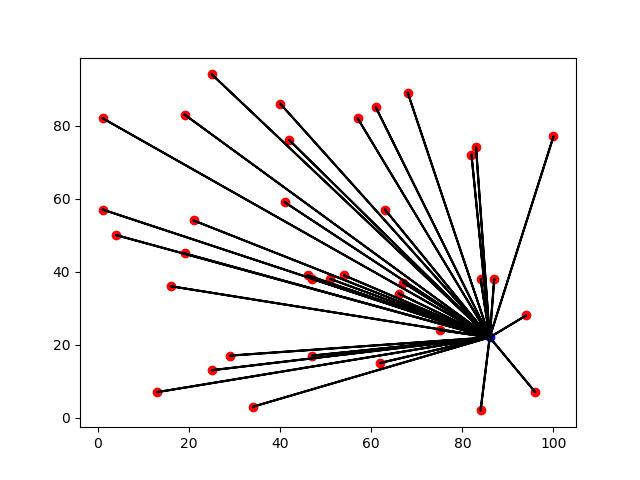
\includegraphics[scale=0.4]{CWinit.png}
  	\caption{Initialisation.}
	\label{CWinit}
    \end{minipage}
    \hfill%
    \begin{minipage}[c]{.46\linewidth}
        \centering
	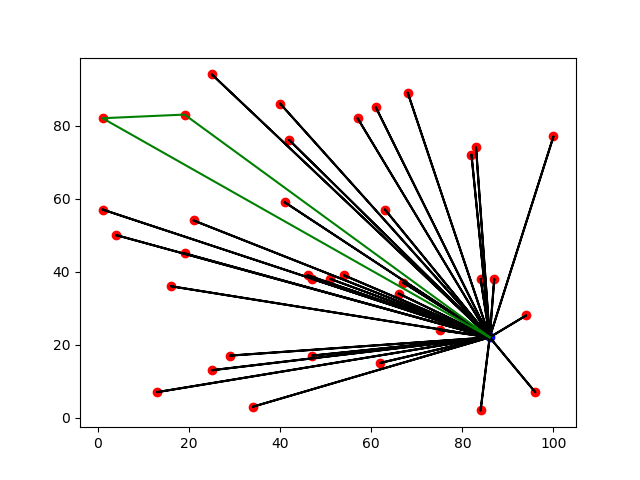
\includegraphics[scale=0.4]{CW1.png}
	\caption{1$^{ere}$ fusion.}
 	\label{CW1}
    \end{minipage}

    \begin{minipage}[c]{.46\linewidth}
        \centering
	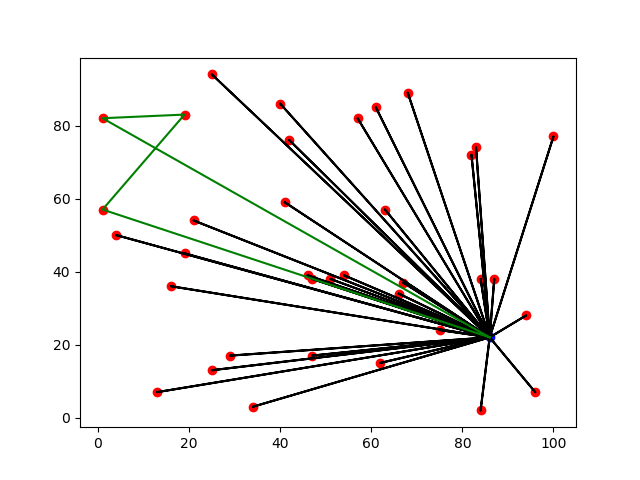
\includegraphics[scale=0.4]{CW2.png}
	\caption{2$^{eme}$ fusion.}
	\label{CW2}
    \end{minipage}
    \hfill%
    \begin{minipage}[c]{.46\linewidth}
        \centering
	 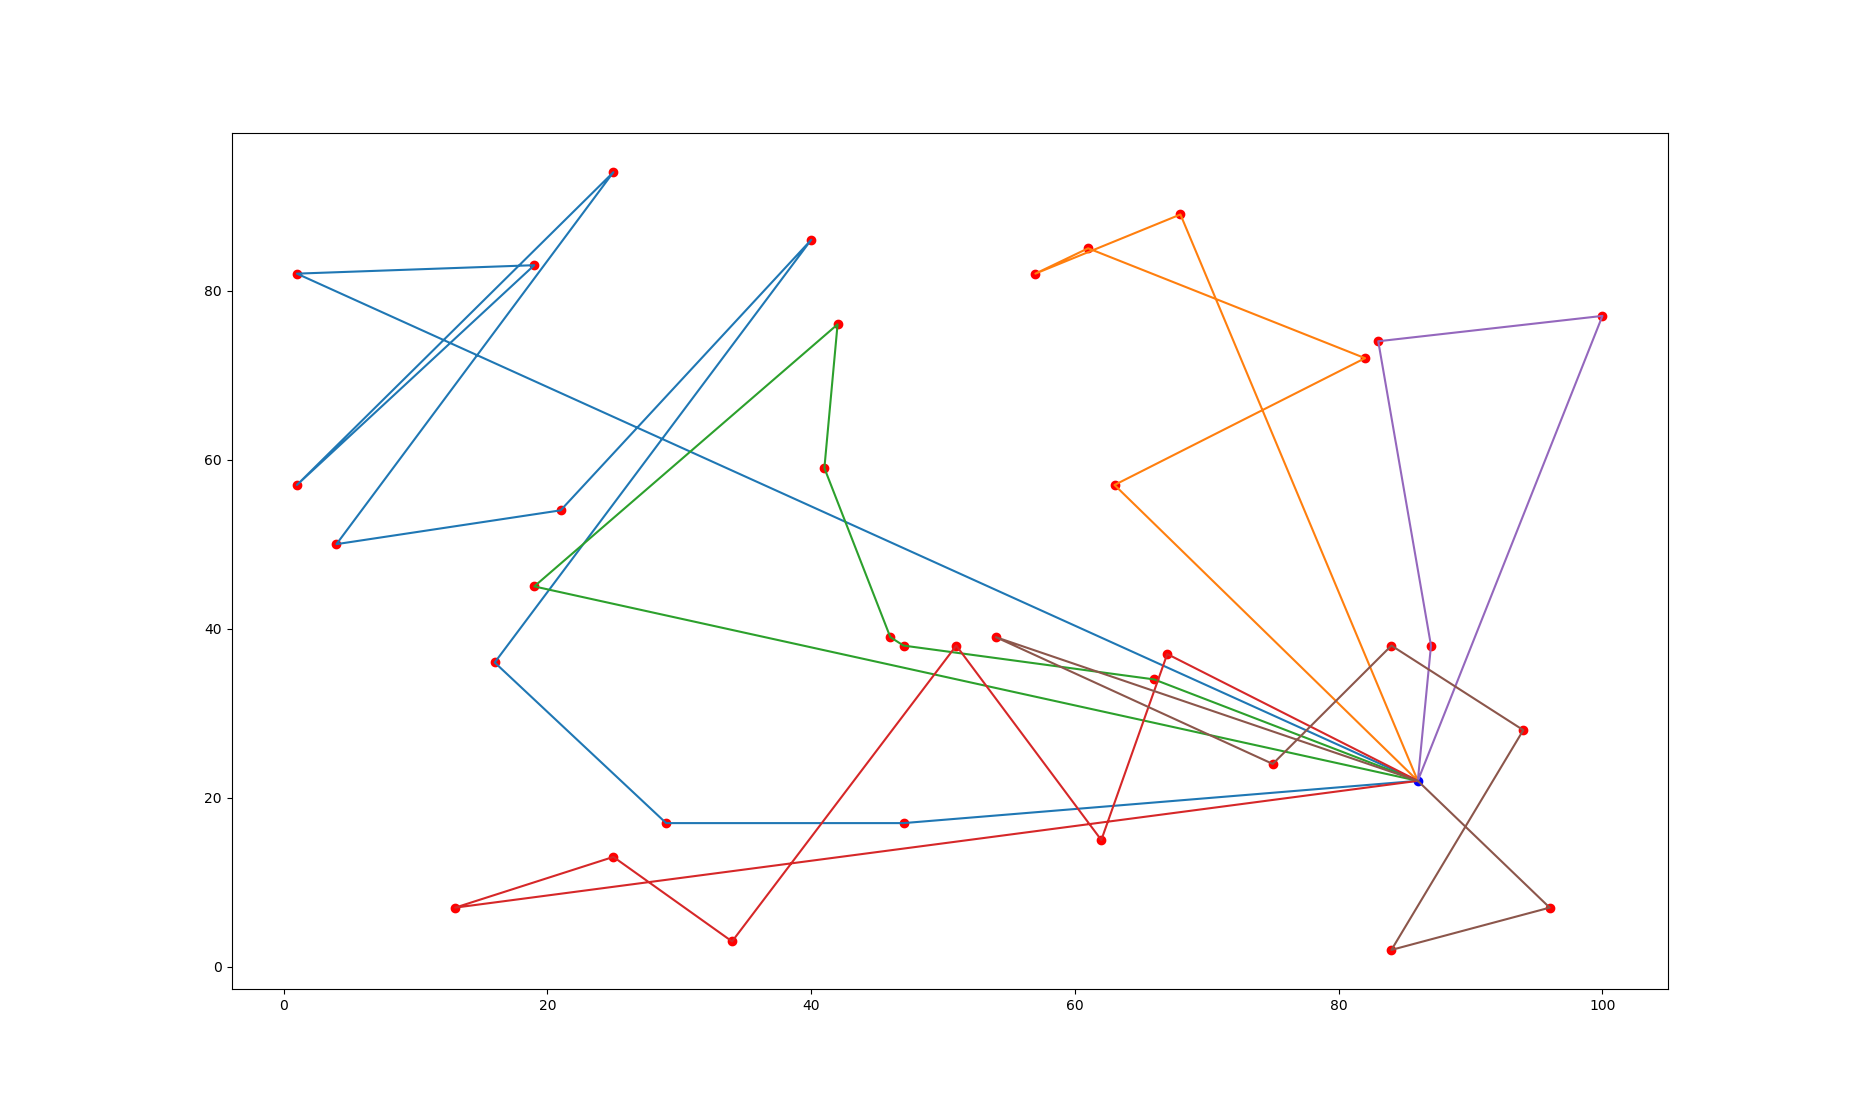
\includegraphics[scale=0.17]{resCW101010.png}
	 \caption{Solution obtenue, $cost = 1297$.}
	\label{resCW101010}
    \end{minipage}
\end{figure}

\subsection{Choix des paramètres $(\lambda, \mu, \nu)$}
Le triplet $(\lambda, \mu, \nu)$ a déjà été étudié de nombreuses fois dans la littérature. L'article~\cite{Altinel_2005} précise qu'il suffit de considérer $(\lambda, \mu, \nu)$ dans $]0,2] \times [0,2]^2$ pour avoir de bonnes solutions. 
Par ailleurs, il est inutile de prendre une précision inférieure au dixième lorsqu'on choisit les valeurs des paramètres.

Les figures \ref{resCW190105} à \ref{resCW001015} présentent différents résultats obtenus pour différents triplets $(\lambda, \mu, \nu)$.
On remarque qu'il n'y a aucun lien entre les résultats et les valeurs de $(\lambda, \mu, \nu)$. 
On ne peut donc pas prévoir à l'avance si le triplet $(\lambda, \mu, \nu)$ va donner un bon résultat ou non.

L'influence de ces paramètres dépend aussi des caractéristiques de l'instance considérée, ainsi on ne peut pas se restreindre au choix d'un triplet qui conviendrait pour toutes les instances. 

\begin{figure}
    \begin{minipage}[c]{.42\linewidth}
        \centering
	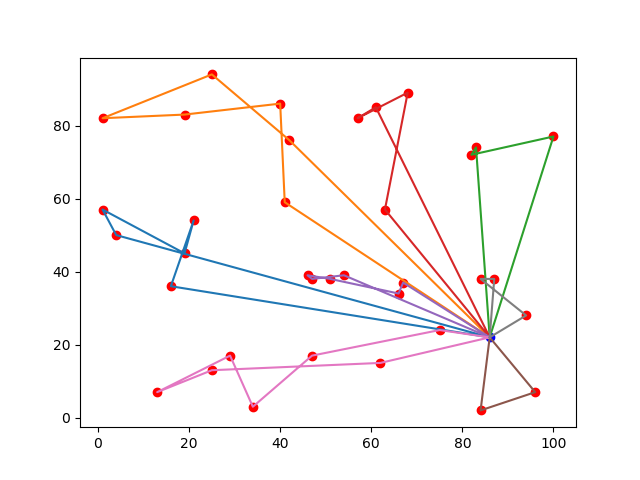
\includegraphics[scale=0.4]{resCW190105.png}
 
 	\caption{$(\lambda, \mu, \nu)=(1.9,0.1,1.5)$, $ cost = 1106$.}
 	\label{resCW190105}
    \end{minipage}
	\hfill%
    \begin{minipage}[c]{.42\linewidth}
        \centering
	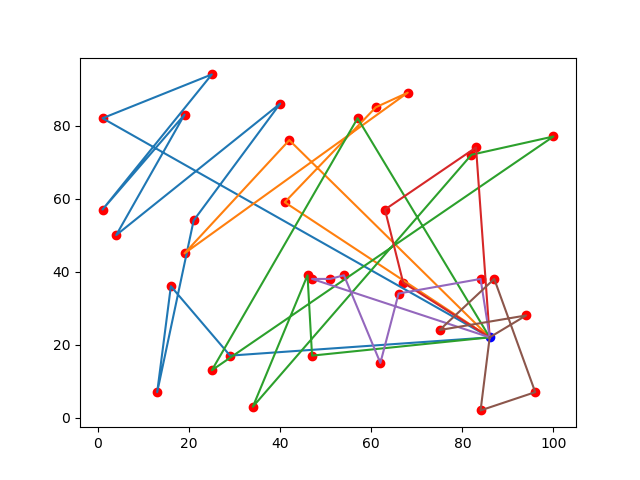
\includegraphics[scale=0.4]{resCW111.png}
	
	\caption{$(\lambda, \mu, \nu)=(0.1,0.1,0.1)$, $cost = 1569$.}
	\label{resCW111}
    \end{minipage}
    
    
        \centering
	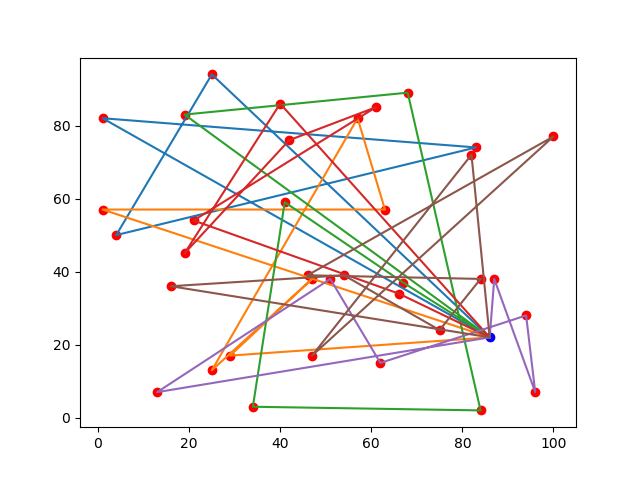
\includegraphics[scale=0.4]{resCW001015.png}
 	\caption{$(\lambda, \mu, \nu)=(0.0,1.0,1.5)$, $cost = 2191$.}
 	\label{resCW001015}
    
\end{figure}

\section{Proposition d'un algorithme d'optimisation}
\label{opti}
Nous proposons dans cette partie un algorithme d'optimisation qui sera utilisé pour y intégrer de la connaissance. Il s'inspire d'un algorithme proposé récemment~\cite{Sorensen_2017}, dont nous détaillons d'abord le fonctionnement, avant de décrire davantage les mécanismes mis en jeu lors de son exécution.

\subsection{Heuristique de Arnold \& Sörensen}
L'heuristique proposée par Arnold et Sörensen~\cite{Sorensen_2017}, est à la fois simple et efficace. 
Il semble donc pertinent de vouloir améliorer cet algorithme en y intégrant de la connaissance.
L'heuristique commence par déterminer une solution initiale via l'algorithme CW, présenté en section~\ref{SolInit}. Différents opérateurs de voisinage sont ensuite appliqués autour d'une arête, considérée comme étant la pire du graphe. Ces opérateurs sont tous en mode $BI-O$ (cf section~\ref{voisinage}), c'est-à-dire que tous les voisins sont parcourus et seul le meilleur est retenu.

L'algorithme~\ref{algo:AS} donne le fonctionnement de l'heuristique (A\&S). 


\begin{algorithm}
\DontPrintSemicolon % Some LaTeX compilers require you to use \dontprintsemicolon instead
\KwIn{Un ensemble de points I, les demandes des clients D, un triplet de flottants $(\lambda,\mu,\nu)$}
\KwOut{Une solution au problème I}
$Sol \gets CW(I,D,\lambda,\mu,\nu)$\;
$N \gets Size(D)$\;
$nextSol \gets Sol$\;
\While {La dernière amélioration date de moins de 3 min} {
	$worstEdge \gets$ Calcul de la pire arête\;
	$nextSol \gets EC_{BI-O}(worstEdge,I,D)$\;
	$nextSol \gets LK_{BI-O}(nextSol)$\;
	$nextSol \gets CE_{BI-O}(worstEdge,I,D)$\;
	$nextSol \gets LK_{BI-O}(nextSol)$\;
	\If {$cost(Sol) > cost (nextSol)$} {
		$ Sol \gets nextSol$\;
	}
	\If {Pas d'améliorations depuis $N/10$ itérations} {
		Appliquer les opérateurs sur toutes les arêtes de la solution\;
	}
	\If {Pas d'améliorations depuis $20N$ itérations} {
		Changer de fonction de pénalisation en prenant un autre triplet $(\gamma_w,\gamma_c,\gamma_d)$\;
	}
	\If {Pas d'améliorations depuis $100N$ itérations} {
		Réinitialiser les pénalités des arêtes\;
	}
}
\Return{$Sol$}\;
\caption{{\sc AS} applique l'heuristique A\& S au problème considéré}
\label{algo:AS}
\end{algorithm}

Les prochaines sections détaillent le calcul de la pire arête, ainsi que le fonctionnement des opérateurs utilisés.


\subsubsection{Pire arête et pénalisation}
Afin de pouvoir comparer les différentes arêtes entre elles et déterminer laquelle est la pire, il faut disposer de certaines métriques sur les arêtes pour pouvoir les caractériser.

Trois métriques sont détaillées dans l'article~\cite{Sorensen_2017}:
\begin{itemize}
\item Le coût d'une arête $(i,j)$, que l'on note $c(i,j)$ se calcule de la manière suivante:

\begin{center}
$c(i,j) = c_{ij}(1 + \beta p(i,j))$ 
\end{center}

Dans l'article~\cite{Sorensen_2017} $\beta = 0.1$. $p(i,j)$ correspond au nombre de fois où l'arête $(i,j)$ a été pénalisé;
\item La profondeur d'une arête $(i,j)$, noté $d(i,j)$ a pour formule :

\begin{center}
max($c_{0i}$, $c_{0j}$)
\end{center}

Autrement dit c'est la distance entre le point le plus éloigné du dépôt et le dépôt.
\item La largeur de l'arête $(i,j)$, noté $w(i,j)$ est la différence de longueur entre les projetés de $i$ et $j$ sur la droite issue du dépôt passant par le centre de gravité de la tournée. Le centre de gravité d'une tournée étant obtenu en faisant la moyenne, pour chaque composante, des points de cette tournée.
\end{itemize}

Les notions de coût, profondeur et largeur sont illustrées par la figure~\ref{metrics}. 

\begin{figure}
\centering
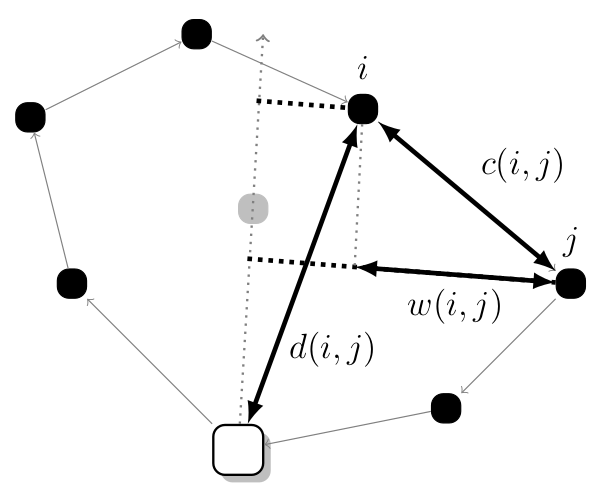
\includegraphics[scale=0.3]{metrics_big.png}
\caption{Illustration des caractéristiques d'une arête.}
\label{metrics}
\end{figure}

On définit alors la fonction de pénalisation $b$ de la manière suivante :
\begin{center}
$b(i,j) = \frac{[\gamma_w w(i,j) + \gamma_c c(i,j)] [\frac{d(i,j)}{max_{k,l}d(k,l)}] ^ {\frac{\gamma_d}{2}}}{1+p(i,j)}$
\end{center}

Les paramètres $\gamma_w,\gamma_c,\gamma_d$, prennent comme valeurs $0$ ou $1$, selon les caractéristiques que l'on veut considérer. 
Il y a ainsi 6 fonctions de pénalisation différentes, que l'on peut choisir au cours de l'exécution (on ne considère pas le cas où $\gamma_w = \gamma_c = 0$, puisqu'il fournit $b(i,j) = 0$.

On peut alors définir ce qu'est la pire arête $(i^*,j^*)$ du graphe :

\begin{center}
$ (i^*,j^*) = argmax_{i,j} b(i,j)$
\end{center}

Les opérateurs de voisinage, présentés ci-après, vont orienter leurs recherches autour de cette pire arête.
 
\subsubsection{Ejection-Chain}

Le premier opérateur utilisé est appelé Ejection-Chain. Son objectif est de déplacer au plus $l$ clients sur des tournées. 

Supposons que l'on veuille supprimer une arête $(c_1^-,c_1)$ d'une tournée $r_1$.
On commence par chercher le plus proche voisin $c_2$ de $c_1$ appartenant à une tournée $r_2$ dans laquelle il est possible d'ajouter $c_1$.
On insère alors $c_1$ après $c_2$ sur $r_2$. 
Ainsi la portion $[...,c_2,c_2^+,...]$ de $r_2$ se transforme en $[...,c_2,c_1,c_2^+,...]$.
On cherche ensuite une arête à supprimer sur $r_2$, pour éjecter un client sur une tournée $r_3$, et ainsi de suite jusqu'à atteindre la tournée $r_l$.
Le fonctionnement de cet opérateur est présenté sur la figure~\ref{EC}. 

\begin{figure}
\centering
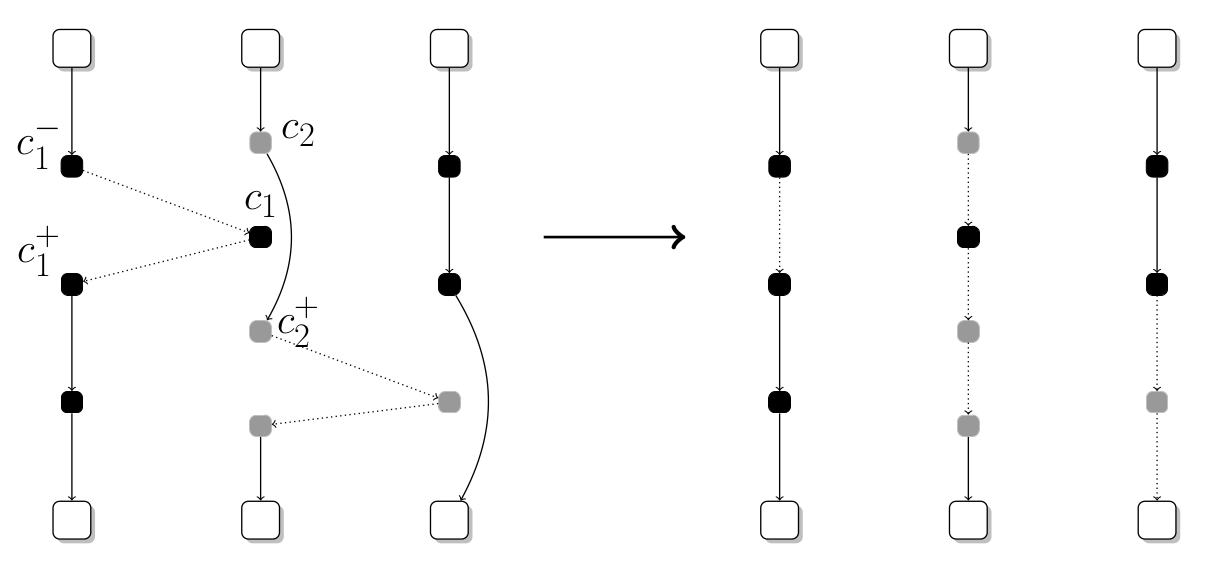
\includegraphics[scale=0.2]{ejection_chain_big.png}
\caption{Exemple de fonctionnement de l'opérateur ejection-chain.}
\label{EC}
\end{figure}

Dans l'article~\cite{Sorensen_2017} $l = 3$. En effet l'algorithme~\ref{algo:EC}, qui décrit le fonctionnement de cet opérateur, s'exécute en $O(n^{l-1})$. Il vaut donc mieux choisir une valeur de $l$ assez petite, pour que la complexité n'explose pas. 

\begin{algorithm}
\DontPrintSemicolon % Some LaTeX compilers require you to use \dontprintsemicolon instead
\KwIn{Une arête $(a,b)$, la liste des plus proches voisins des clients $voisins$, un entier $l$, la solution actuelle $sol$}
\KwOut{Une nouvelle solution au moins aussi bonne que $sol$}
$possibleSol \gets sol$\;
$cand \gets choose(a,b)$\;
$nextRoute \gets findNextRoute(cand,voisins,possibleSol)$\;
$possibleSol \gets $ déplacer $cand$ après son voisin sur $nextRoute$\;
\For{$i \gets 1$ \textbf{to} $l-1$} {
  $cand \gets $un client de $nextRoute$ différent de celui ajouté\;
  $nextRoute \gets findNextRoute(cand,voisins,possibleSol)$\;
  $possibleSol \gets$ déplacer $cand$ après son voisin sur $nextRoute$\;
}
\If {$cost(possibleSol) < cost(sol)$} {
	$sol \gets possibleSol$\;
}
\Return{$sol$}\;
\caption{{\sc Ejection-Chain} applique l'opérateur ejection-chain}
\label{algo:EC}
\end{algorithm}

Aux lignes $3, 4, 7$ et $8$ de l'algorithme~\ref{algo:EC}, il est possible d'utiliser les méthodes de la section~\ref{voisinage} pour explorer les voisinages.

\subsubsection{Cross-Exchange}

Un deuxième opérateur utilisé est le Cross-Exchange.
Son objectif est d'échanger deux séquences de clients entre deux tournées.

Supposons que l'on veuille supprimer une arête $(c_1,c_2)$ appartenant à une tournée $r_1$. 
On cherche le plus proche voisin $c_4$ de $c_1$ appartenant à une tournée $r_2$.
On échange alors $c_1$ avec le prédécesseur $c_3$ de $c_4$.
Il suffit ensuite de considérer deux autres clients entre les deux tournées, pour  échanger deux séquences de clients.
Le fonctionnement de cet opérateur est présenté sur la figure~\ref{CE}.

\begin{figure}
\centering
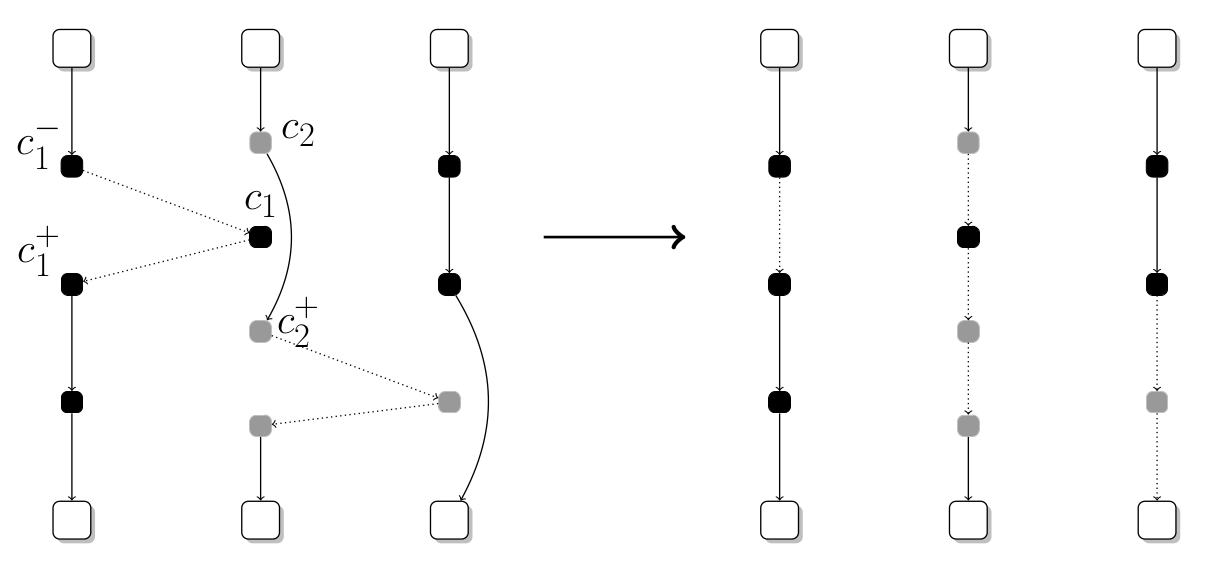
\includegraphics[scale=0.2]{cross_exchange_big.png}
\caption{Exemple de fonctionnement de l'opérateur cross-exchange.}
\label{CE}
\end{figure}

Il est possible de limiter le nombre de clients par séquence échangée.
L'algorithme~\ref{algo:CE} présente l'exécution de l'opérateur et s'exécute en $O(n^2)$.

\begin{algorithm}
\DontPrintSemicolon 
\KwIn{Une arête $(c_1,c_2)$, la liste des plus proches voisins des clients $voisins$, la solution actuelle $sol$}
\KwOut{Une nouvelle solution au moins aussi bonne que $sol$}
$possibleSol \gets sol$\;
$nextRoute \gets findNextRoute(c_1,voisins,possibleSol)$\;
Considérer l'arête $(c_3,c_4)$ de $nextRoute$, où $c_4$ est le proche voisin de $c_1$ utilisé\;
$possibleSol \gets exchange(c_1,c_3,possibleSol)$\;
Choisir 2 clients $c_5$ et $c_6$ qui n'appartiennent pas à la même tournée\;
$possibleSol \gets exchange(c_5,c_6,possibleSol)$\;
\If {$cost(possibleSol) < cost(sol)$} {
	$sol \gets possibleSol$\;
}
\Return{$sol$}\;
\caption{{\sc Cross-Exchange} applique l'opérateur cross-exchange}
\label{algo:CE}
\end{algorithm}

A la ligne $6$ de l'algorithme~\ref{algo:CE}, il est possible d'utiliser les méthodes de la section \ref{voisinage} pour explorer les voisinages, et choisir les clients à échanger.

\subsubsection{Lin-Kernighan}
\label{Lin-Kernighan}
Le dernier opérateur utilisé est l'heuristique Lin-Kernighan. Elle a été créée pour résoudre le problème du voyageur de commerce (TSP). 
Il effectue une optimisation intra-tournée (c'est-à-dire que la tournée considérée est améliorée indépendamment des autres).
Cela consiste en une réorganisation des clients sur la tournée. On choisit $k$ tel que \emph{LK} ne dépasse pas \emph{k-opt} au cours de son exécution. 
On appelle \emph{k-opt}, l'opération qui consiste à échanger $k$ clients différents sur la tournée.

On commence alors par appliquer 2-opt, si une amélioration est trouvée, on passe à 3-opt, et ainsi de suite jusqu'à atteindre k-opt. 
On repart alors de 2-opt, et ce jusqu'à ne plus trouver d'améliorations, comme le décrit l'algorithme~\ref{algo:LK}.
D'après l'article~\cite{Sorensen_2017}, on peut prendre $k = 2$.
 
Un exemple d'utilisation de cet opérateur est présent sur la figure~\ref{LK}

\begin{figure}
\centering
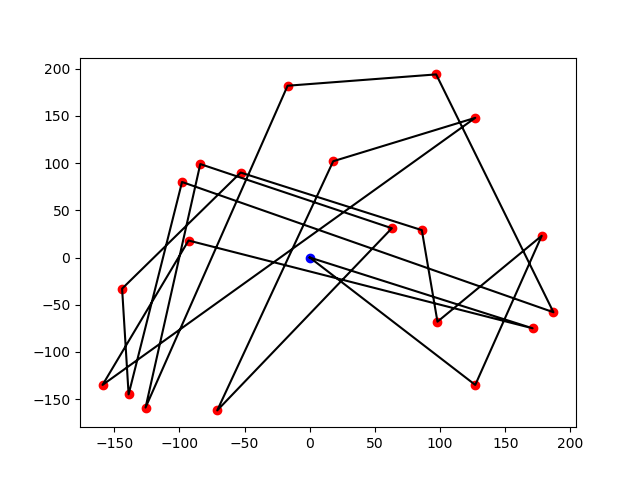
\includegraphics[scale=0.4]{test4_20_init.png}
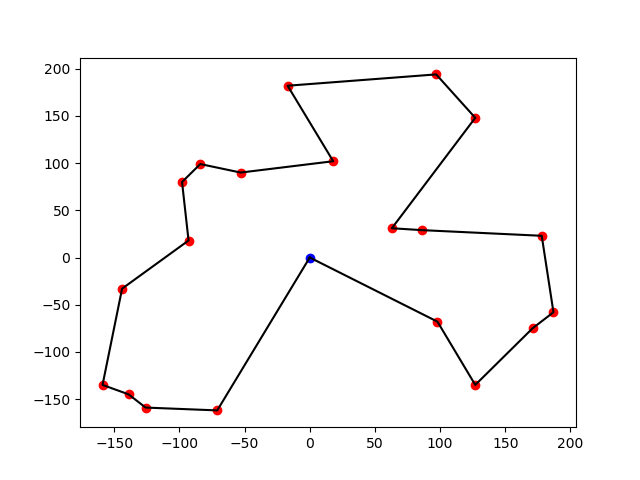
\includegraphics[scale=0.4]{test4_20_LKopt.png}

\caption{Exemple de fonctionnement de l'opérateur LK.}
\label{LK}
\end{figure}

\begin{algorithm}
\DontPrintSemicolon % Some LaTeX compilers require you to use \dontprintsemicolon instead
\KwIn{Une tournée $r$ à améliorer}
\KwOut{Une permutation de $r$ ayant un meilleur coût que $r$}
$r_{next} \gets 2$-$opt(r) $\;
\While{$ r_{next} \neq r$} {
  $r \gets r_{next}$\;
  $r_{next} \gets 2$-$opt(r)$\;
}
\Return{$r$}\;
\caption{{\sc Lin-Kernighan} applique l'opérateur Lin-Kernighan}
\label{algo:LK}
\end{algorithm}

Lorsqu'il s'agit d'appliquer \emph{2-opt}, il est possible d'utiliser les méthodes de la section \ref{voisinage} pour explorer les voisinages.

\subsection{Algorithme d'optimisation utilisé}
L'algorithme d'optimisation que nous utilisons est un peu différent de l'heuristique A\&S précédente.

Pour diminuer le temps d'exécution, nous choisissons de diminuer le temps limite entre deux nouvelles solutions à $limitTime$ secondes. 
Pour que l'exploration du voisinage des solutions soit plus efficace, nous décidons de passer les opérateurs \emph{EC} et \emph{CE} en mode $FI-RD$ (ce qui est généralement le cas dans les algorithmes d'optimisation).
Enfin, nous ajoutons une condition de \emph{Restart}, s'il n'y a pas eu d'améliorations depuis \emph{restartTime} secondes.

L'algorithme~\ref{algo:HC} présente en gras les changements effectués, par rapport à l'algorithme~\ref{algo:AS}.

\begin{algorithm}
\DontPrintSemicolon % Some LaTeX compilers require you to use \dontprintsemicolon instead
\KwIn{Un ensemble de points I, les demandes des clients D, un triplet de flottants $(\lambda,\mu,\nu)$}
\KwOut{Une solution au problème I}
$Sol \gets CW(I,D,\lambda,\mu,\nu)$\;
$N \gets length(D)$\;
$nextSol \gets Sol$\;
\While {La dernière amélioration date de moins de \textbf{limitTime} secondes} {
	$worstEdge \gets argmax_{(i,j)} b(i,j) $\;
	$nextSol \gets EC_{\textbf{FI-RD}}(worstEdge,I,D)$\;
	$nextSol \gets LK_{BI-O}(nextSol)$\;
	$nextSol \gets CE_{\textbf{FI-RD}}(worstEdge,I,D)$\;
	$nextSol \gets LK_{BI-O}(nextSol)$\;
	\If {$cost(Sol) > cost (nextSol)$} {
		$ Sol \gets nextSol$\;
	}
	
	\If {\textbf{Pas d'améliorations depuis \textbf{restartTime} secondes}} {
		$nextSol \gets Sol$\;
	
	}
	
	\If {\textbf{Pas d'améliorations depuis \textbf{resetTime} secondes}} {
		Changer de fonction de pénalisation en prenant un autre triplet $(\gamma_w,\gamma_c,\gamma_d)$\;
		Réinitialiser les pénalités des arêtes\;
	}
	
}
\Return{$Sol$}\;
\caption{{\sc $H_c$} calcule une solution du problème considéré}
\label{algo:HC}
\end{algorithm}

Nous pouvons à présent nous intéresser à l'extraction des connaissances des solutions initiales.

\section{Extraction de la connaissance}
\label{extraction}
Cette section s'intéresse à l'extraction de connaissance à partir de solutions initiales générées. 
Nous expliquons dans un premier temps quelle va être la connaissance extraite des solutions initiales, puis nous décrivons notre protocole d'apprentissage ainsi que les problématiques qu'il soulève.
Enfin, nous présentons quelques résultats obtenus, servant à déterminer les paramètres choisis lors de l'apprentissage. 

\subsection{Quelle est la connaissance ?}

En observant quelques solutions obtenues avec \emph{CW}, auxquelles est appliquée l'opérateur \emph{LK}, on remarque que plus la solution initiale est bonne et plus elle possède d'arêtes en commun avec la solution optimale. 

Ce résultat est illustré sur les figures~\ref{edges190115} à \ref{edgesSol}, où les arêtes optimales sont vertes.


\begin{figure}
    \begin{minipage}[c]{.46\linewidth}
        \centering
  	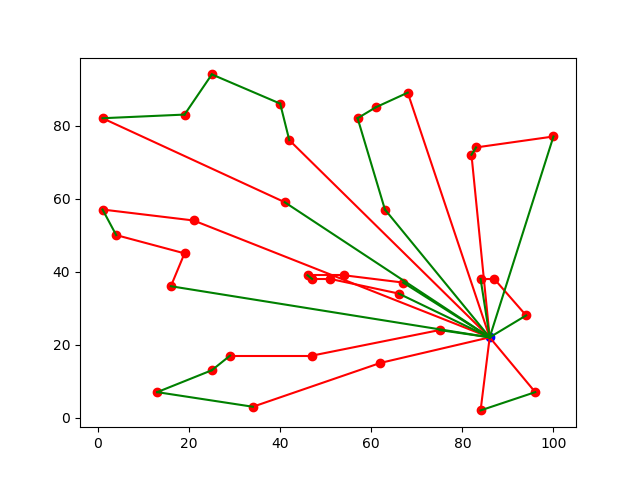
\includegraphics[scale=0.4]{edges190115.png}
	\caption{$CW(1.9,0.1,1.5)+LK$, $cost = 1041$, 19 arêtes optimales.}
	\label{edges190115}
    \end{minipage}
    \hfill%
    \begin{minipage}[c]{.46\linewidth}
        \centering
	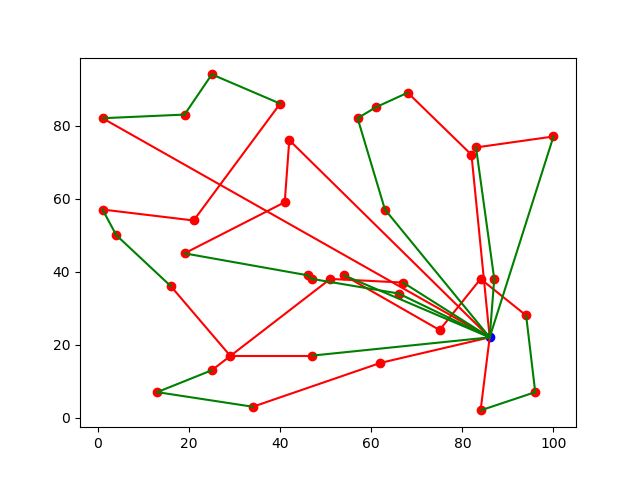
\includegraphics[scale=0.4]{edges101010.png}
	\caption{$CW(0.1,0.1,0.1)+LK$, $cost = 1170$, 19 arêtes optimales.}
	\label{edges101010}
    \end{minipage}

    \begin{minipage}[c]{.46\linewidth}
        \centering
	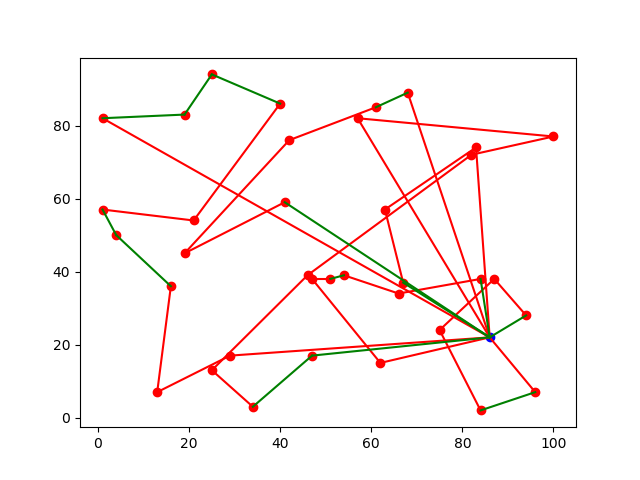
\includegraphics[scale=0.4]{edges010101.png}
	\caption{$CW(0.0,1.0,1.5)+LK$, $cost = 1600$, 11 arêtes optimales.}
	\label{edges010101}	
    \end{minipage}
    \hfill%
    \begin{minipage}[c]{.46\linewidth}
        \centering
	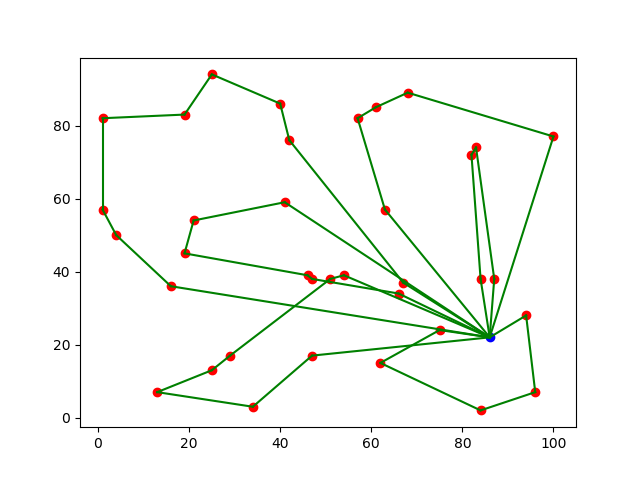
\includegraphics[scale=0.4]{edgesSol.png}
	\caption{Solution optimale, 42 arêtes.}
	\label{edgesSol}
    \end{minipage}
\end{figure}

Il faudrait donc pouvoir déterminer à l'avance les arêtes optimales à partir des solutions initiales fournies par l'utilisation de \emph{CW} suivi de \emph{LK}.

\subsection{Protocole d'apprentissage}
Pour extraire cette connaissance, nous allons devoir créer un échantillon de solutions initiales, à partir duquel nous allons extraire une base d'apprentissage. Cette base va nous permettre d'extraire des arêtes. Afin de vérifier nos résultats, nous comparerons les arêtes obtenues aux arêtes de la solution optimale.

\subsubsection{Génération de l'échantillon}
Puisque l'on ne peut pas prédire les paramètres $(\lambda,\mu,\nu)$ pour obtenir de bonnes solutions, nous allons devoir en générer un certain nombre :

\begin{itemize}
\item Soit on génère l'intégralité des solutions initiales possibles, en parcourant tous les triplets $(\lambda,\mu,\nu)$ (i.e. génération de 8820 solutions), pour obtenir l'échantillon. On l'appelle échantillon \emph{complet};
\item Soit on tire $N$ triplets $(\lambda,\mu,\nu)$ aléatoirement, et les solutions obtenus constitueront notre échantillon. 
\end{itemize}

Les solutions qui constituent notre échantillon ne sont pas nécessairement toutes différentes.
On appelle $c_{min}$ et $c_{max}$ les coûts respectifs de la meilleure et de la pire solution, obtenues dans l'échantillon. 

Nous nous intéressons à présent, à la construction d'une base d'apprentissage.

\subsubsection{Construction de la base d'apprentissage}
La base d'apprentissage, contiendra toutes les solutions utilisées ensuite pour apprendre. Cette base correspond à un sous-ensemble de l'échantillon obtenu. 
Nous avons retenu trois manières différentes pour obtenir cette base :

\begin{itemize}
\item On conserve l'intégralité de l'échantillon. On appelle cette base \emph{Tout};
\item On conserve $x\%$ des meilleures solutions. Dans ce cas, on dit qu'on privilégie la quantité. On appelle cette base \emph{Quan$_x$};
\item On conserve les solutions qui ont un coût inférieur à $c_{min} + (c_{max}-c_{min})\frac{x}{100}$. Dans ce cas, on dit qu'on privilégie la qualité. On appelle cette base \emph{Qual$_x$}.
\end{itemize}

Avec cette base d'apprentissage, nous allons extraire des arêtes qui ont de grandes chances d'être optimales (i.e. qui appartiennent à la solution optimale).

\subsubsection{Extraction des arêtes}
Avant tout, nous considérons que les arêtes $(i,j)$ et $(j,i)$ sont identiques (ce qui est le cas en pratique). Chaque arêtes $(i,j)$ a donc pour représentant $(i',j')$, avec $(i',j') = (i,j)$ si $i<j$, et $(i',j') = (j,i)$ sinon.

Pour savoir si une arête $(i,j)$ est souvent prise dans les solutions de notre base d'apprentissage, nous incrémentons la valeur $Learn[i][j]$ d'une matrice $Learn$ de taille $n^2$ (initialement nulle), lorsque cette arête appartient à la solution considérée.
Une fois toutes les solutions parcourues, nous avons retenu deux critères pour extraire les arêtes potentiellement intéressantes :

\begin{itemize}
\item Soit nous conservons les $rang$ premières arêtes (pour les valeurs de $Learn$). On appelle ce critère \emph{Rang};
\item Soit nous conservons $(i,j) \Leftrightarrow Learn[i][j] > seuil$. On appelle ce critère \emph{Seuil}.
\end{itemize}

Afin de déterminer quels doivent être la taille de l'échantillon, la base d'apprentissage, ainsi que le critère utilisé, la partie suivante présente les résultats obtenus.

\subsection{Résultats}


\subsubsection{Choix de l'échantillon et de la base}

On choisit de prendre les valeurs suivantes :

\begin{itemize}
\item Taille de l'échantillon : $N \in [50,100,500]$ et \emph{complet}
\item Base d'apprentissage : $Base \in [Tout, Quan_{10}, Qual_{10}]$
\item Critères : $rang \in [10,20,n/2]$ et $seuil \in [\vert Base \vert /2, 3\vert Base \vert /4]$.
\end{itemize}

L'apprentissage est réalisé sur trois instances de tailles différentes : \emph{A-n37-k06}, \emph{A-n65-k09} et \emph{P-n101-k04}. Les figures~\ref{A3706} à~\ref{solP10104}, présentent les trois instances, ainsi que les solutions optimales associées. 

Les résultats obtenus pour chaque instance est présenté dans un tableau (cf tableaux~\ref{T1} à~\ref{T3}). Ils correspondent aux moyennes obtenus sur $10$ échantillons de la taille considérée.
La colonne \emph{Arêtes} donne le nombre d'arêtes obtenues. 
La colonne  \emph{Optimales} donne le nombre d'arêtes qui appartiennent effectivement à la solution optimale.
Enfin, la colonne \emph{Prop}, donne la proportion d'arêtes optimales parmi toutes les arêtes de la solution optimale. 

\begin{figure}[h!]
    \begin{minipage}[c]{.46\linewidth}

        \centering
        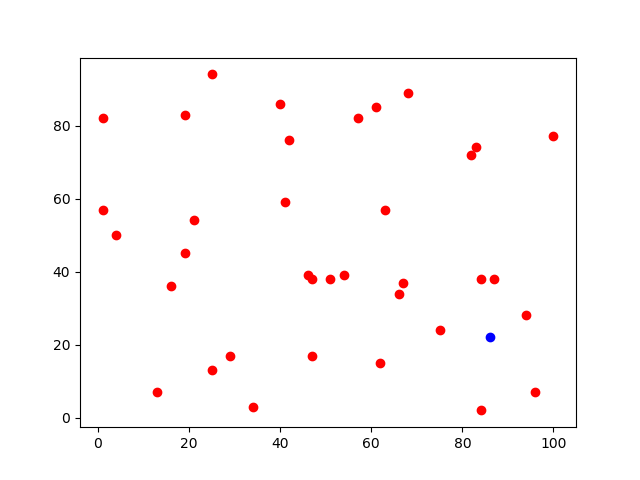
\includegraphics[scale=0.4]{instance3706}
        
        \caption{Instance \emph{A-n37-k06}.}
        \label{A3706}

    \end{minipage}
    \hfill%
    \begin{minipage}[c]{.46\linewidth}
        \centering
        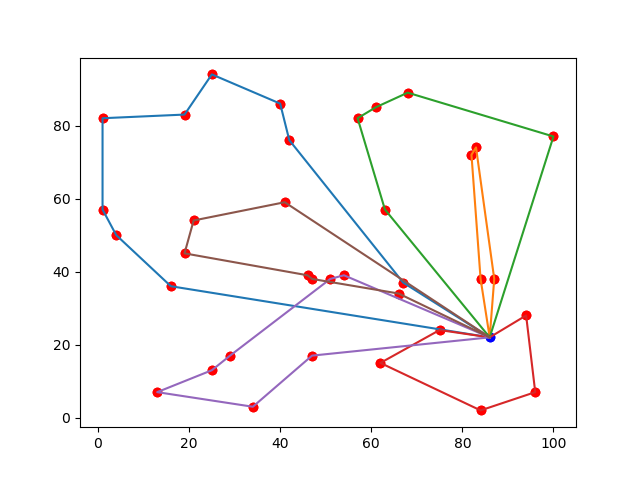
\includegraphics[scale=0.4]{best3706}
        
        \caption{Solution optimale \emph{A-n37-k06}, 42 arêtes.}
        \label{SolA3706}
    \end{minipage}
    
    \begin{minipage}[c]{.46\linewidth}
        \centering
        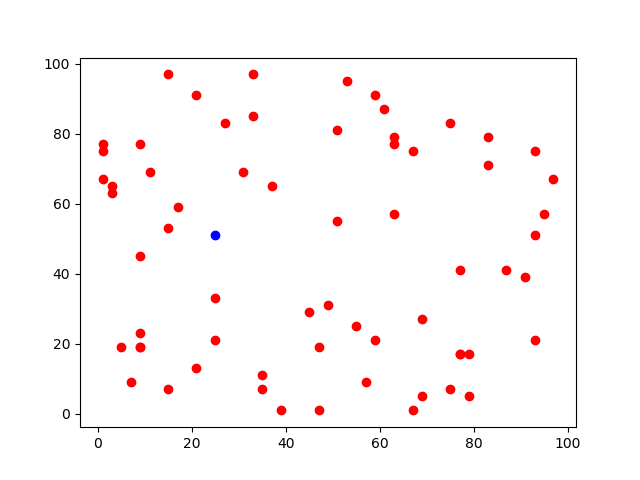
\includegraphics[scale=0.4]{Instance6509}
        
        \caption{Instance \emph{A-n65-k09}.}
        \label{A6509}
    \end{minipage}
    \hfill%
    \begin{minipage}[c]{.46\linewidth}
        \centering
        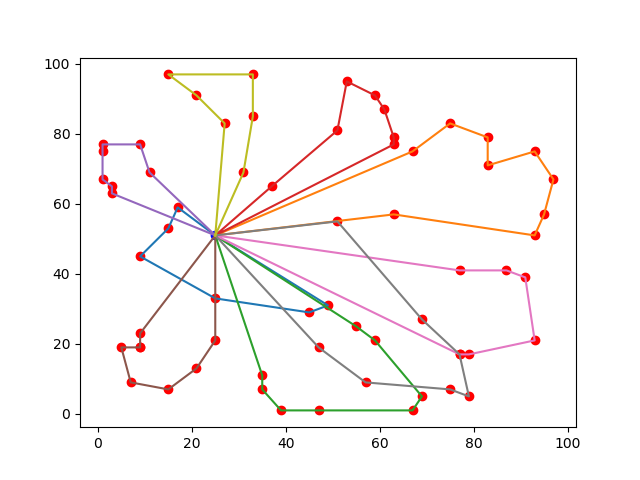
\includegraphics[scale=0.4]{Solution6509}
        
        \caption{Solution optimale \emph{A-n65-k09}, 73 arêtes.}
        \label{SolA6509}
    \end{minipage}    
    
        \begin{minipage}[c]{.46\linewidth}
        \centering
        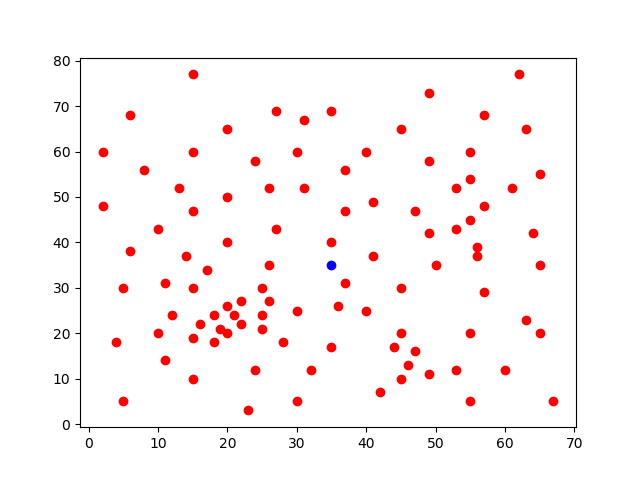
\includegraphics[scale=0.4]{Instance10104}
        
        \caption{Instance \emph{P-n101-k04}.}
        \label{P10104}
    \end{minipage}
    \hfill%
    \begin{minipage}[c]{.46\linewidth}
        \centering
        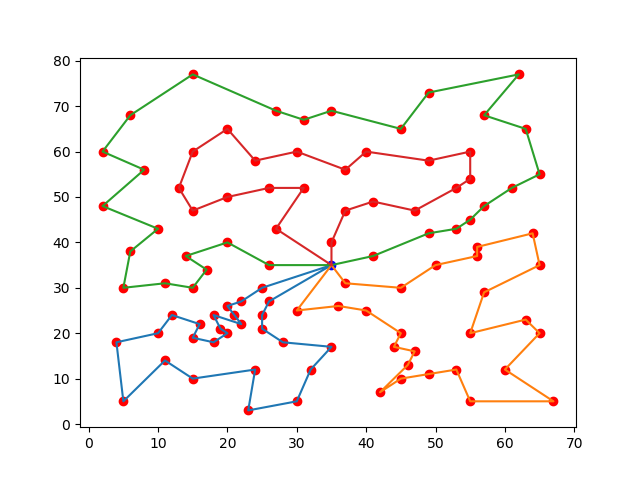
\includegraphics[scale=0.4]{Solution10104}
        
        \caption{Solution optimale \emph{P-n101-k04}, 104 arêtes.}
        \label{solP10104}
    \end{minipage}
\end{figure}

\begin{table}[h]
\caption{Résultats pour l'instance \emph{A-n37-k06}}
\label{T1}
\begin{center}
\begin{tabular}{|@{}c@{}|@{}c@{}|@{}c@{}|@{}c@{}|@{}c@{}||@{}c@{}|@{}c@{}|@{}c@{}|@{}c@{}||@{}c@{}|@{}c@{}|@{}c@{}|@{}c@{}|}

\hline
 Échantillon & \multicolumn{4}{c|}{Quan$_{10}$} & \multicolumn{4}{c|}{Qual$_{10}$} & \multicolumn{4}{c|}{Tout} \\
 \hline
 & Seuil & Arêtes & Optimales & Prop & Seuil & Arêtes & Optimales & Prop & Seuil & Arêtes & Optimales & Prop \\
 \hline
 50 & 3 & 34 & 21 & 0.5 & 11 & 33 & 21 & 0.50 & 25 & 23 & 15 & 0.35 \\
 \cline{2-13} 
    & 4 & 23 & 14 & 0.33 & 17 & 17 & 12 & 0.28 & 38 & 10 & 7 & 0.16 \\
  \hline
   100 & 5 & 30 & 21 & 0.5 & 15 & 31 & 23 & 0.55 & 50 & 24 & 17 & 0.40 \\
 \cline{2-13} 
    & 8 & 16 & 15 & 0.36 & 23 & 17 & 14 & 0.33 & 75 & 6 & 6 & 0.14 \\
  \hline
   500 & 25 & 32 & 24 & 0.57 & 58 & 31 & 22 & 0.52 & 250 & 22 & 15 & 0.36 \\
 \cline{2-13} 
    & 38 & 15 & 14 & 0.33 & 88 & 20 & 16 & 0.38 & 375 & 7 & 7 & 0.18 \\
  \hline
   Complet & 400 & 33 & 24 & 0.57 & 732 & 30 & 23 & 0.55 & 4000 & 25 & 16 & 0.38 \\
 \cline{2-13} 
    & 600 & 15 & 14 & 0.33 & 1097 & 18 & 16 & 0.38 & 6000 & 9 & 6 & 0.14 \\
  \hline
  \hline
 & Rang & Arêtes & Optimales & Prop & Rang&Arêtes & Optimales & Prop & Rang &Arêtes& Optimales & Prop \\
 \hline
 50 & 10 &  & 6 & 0.14 & 10&  & 6 & 0.14 & 10&  & 7 & 0.16  \\
 \cline{2-13} 
    & 20& & 13 & 0.31 & 20&  & 13 & 0.32 & 20&  & 13 & 0.31  \\
 \cline{2-13} 
    & 18& & 12 & 0.28 & 18& & 13 & 0.3 & 18& & 12 & 0.28  \\
  \hline
   100 & 10&  & 9 & 0.21 & 10&  & 9 & 0.21 & 10&  & 10 & 0.24  \\
 \cline{2-13} 
    & 20& & 16 & 0.38 & 20& & 16 & 0.38 & 20& & 15 & 0.36  \\
  \cline{2-13} 
    & 18& & 13 & 0.3 & 18& & 13 & 0.3 & 18& & 12 & 0.29  \\
  \hline
   500 & 10&  & 9 & 0.21 & 10&  & 10 & 0.24 & 10&  & 9 & 0.21  \\
 \cline{2-13} 
    & 20& & 16 & 0.38 & 20& & 16 & 0.38 & 20& & 15 & 0.36  \\
  \cline{2-13} 
    & 18& & 13 & 0.3 & 18& & 13 & 0.3 & 18& & 12 & 0.28  \\
  \hline
   Complet & 10& & 8 & 0.19&  10& & 9 & 0.21 & 10& & 7 & 0.17  \\
 \cline{2-13} 
    & 20& & 14 & 0.33 & 20& & 14 & 0.33 & 20& & 14 & 0.33  \\
  \cline{2-13} 
    & 18& & 12 & 0.29 & 18& & 12 & 0.29 & 18& & 12 & 0.29  \\
  \hline
  
\end{tabular}
\end{center}
\end{table}


\begin{table}[h]
\caption{Résultats pour l'instance \emph{A-n65-k09}}
\label{T2}
\begin{center}
\begin{tabular}{|@{}c@{}|@{}c@{}|@{}c@{}|@{}c@{}|@{}c@{}||@{}c@{}|@{}c@{}|@{}c@{}|@{}c@{}||@{}c@{}|@{}c@{}|@{}c@{}|@{}c@{}|}

\hline
 Échantillon & \multicolumn{4}{c|}{Quan$_{10}$} & \multicolumn{4}{c|}{Qual$_{10}$} & \multicolumn{4}{c|}{Tout} \\
 \hline
 & Seuil & Arêtes & Optimales & Prop & Seuil & Arêtes & Optimales & Prop & Seuil & Arêtes & Optimales & Prop \\
 \hline
 50 & 3 & 73 & 43 & 0.59 & 10 & 64 & 44 & 0.60 & 25 & 40 & 31 & 0.43 \\
 \cline{2-13} 
    & 4 & 61 & 40 & 0.55 & 15 & 39 & 29 & 0.40 & 38 & 14 & 9 & 0.13 \\
  \hline
   100 & 5 & 70 & 44 & 0.6 & 22 & 58 & 42 & 0.58 & 50 & 43 & 33 & 0.45 \\
 \cline{2-13} 
    & 8 & 63 & 41 & 0.56 & 33 & 36 & 28 & 0.39 & 75 & 15 & 10 & 0.14 \\
  \hline
   500 & 25 & 71 & 43 & 0.59 & 111 & 56 & 41 & 0.56 & 250 & 45 & 35 & 0.48 \\
 \cline{2-13} 
    & 38 & 60 & 40 & 0.55 & 167 & 35 & 28 & 0.39 & 375 & 14 & 9 & 0.13 \\
  \hline
   Complet & 400 & 62 & 41 & 0.56 & 1005 & 56 & 40 & 0.55 & 4000 & 45 & 35 & 0.48 \\
 \cline{2-13} 
    & 600 & 15 & 14 & 0.33 & 1508 & 35 & 28 & 0.39 & 6000 & 13 & 9 & 0.12 \\
  \hline
 & Rang& Arêtes & Optimales & Prop & Rang& Arêtes & Optimales & Prop & Rang& Arêtes & Optimales & Prop \\
 \hline
 50 & 10 & & 6 & 0.08 & 10&  & 7 & 0.1 & 10&  & 7 & 0.1  \\
 \cline{2-13} 
    & 20& & 14 & 0.2 & 20&  & 15 & 0.21 & 20&  & 14 & 0.19  \\
 \cline{2-13} 
    & 33& & 23 & 0.32 & 33& & 26 & 0.36 & 33& & 24 & 0.33  \\
  \hline
   100 & 10&  & 6 & 0.08 & 10&  & 7 & 0.1 & 10&  & 7 & 0.1  \\
 \cline{2-13} 
    & 20& & 16 & 0.22 & 20& & 16 & 0.22 & 20& & 14 & 0.19  \\
  \cline{2-13} 
    & 33& & 26 & 0.36 & 33& & 26 & 0.36 & 33& & 25 & 0.34  \\
  \hline
   500 & 10&  & 7 & 0.1 & 10&  & 7 & 0.1 & 10&  & 6 & 0.08  \\
 \cline{2-13} 
    & 20& & 17 & 0.23 & 20& & 15 & 0.21 & 20& & 13 & 0.18  \\
  \cline{2-13} 
    & 33& & 27 & 0.37 & 33& & 26 & 0.36 & 33& & 25 & 0.34  \\
  \hline
   Complet & 10& & 7 & 0.1 & 10& & 7 & 0.1 & 10& & 6 & 0.08  \\
 \cline{2-13} 
    & 20& & 17 & 0.23 & 20& & 17 & 0.23 & 20& & 13 & 0.18  \\
  \cline{2-13} 
    & 33& & 27 & 0.37 & 33& & 27 & 0.37 & 33& & 25 & 0.34  \\
  \hline
\end{tabular}
\end{center}
\end{table}

\begin{table}
\caption{Résultats pour l'instance \emph{P-n101-k04}}
\label{T3}
\begin{center}
\begin{tabular}{|@{}c@{}|@{}c@{}|@{}c@{}|@{}c@{}|@{}c@{}||@{}c@{}|@{}c@{}|@{}c@{}|@{}c@{}||@{}c@{}|@{}c@{}|@{}c@{}|@{}c@{}|}

\hline
 Échantillon & \multicolumn{4}{c|}{Quan$_{10}$} & \multicolumn{4}{c|}{Qual$_{10}$} & \multicolumn{4}{c|}{Tout} \\
 \hline
 & Seuil & Arêtes & Optimales & Prop & Seuil & Arêtes & Optimales & Prop & Seuil & Arêtes & Optimales & Prop \\
 \hline
 50 & 3 & 93 & 65 & 0.62 & 5 & 83 & 66 & 0.64 & 25 & 71 & 61 & 0.59 \\
 \cline{2-13} 
    & 4 & 54 & 44 & 0.42 & 8 & 42 & 37 & 0.36 & 38 & 24 & 21 & 0.20  \\
  \hline
   100 & 5 & 80 & 66 & 0.64 & 9 & 79 & 66 & 0.63 & 50 & 72 & 62 & 0.60 \\
 \cline{2-13} 
    & 8 & 45 & 41 & 0.40 & 14 & 42 & 39 & 0.38 & 75 & 24 & 22 & 0.21 \\
  \hline
   500 & 25 & 83 & 69 & 0.67 & 44 & 81 & 68 & 0.66 & 250 & 72 & 63 & 0.60 \\
 \cline{2-13} 
    & 38 & 43 & 39 & 0.38 & 67 & 39 & 36 & 0.35 & 375 & 22 & 20 & 0.19 \\
  \hline
   Complet & 400 & 87 & 73 & 0.7 & 411 & 85 & 71 & 0.68 & 4000 & 70 & 60 & 0.58 \\
 \cline{2-13} 
    & 600 & 42 & 39 & 0.38 & 616 & 41 & 38 & 0.37 & 6000 & 23 & 21 & 0.2 \\
  \hline
 & Rang& Arêtes & Optimales & Prop & Rang& Arêtes & Optimales & Prop & Rang& Arêtes & Optimales & Prop \\
 \hline
 50 & 10&  & 8 & 0.08 & 10&  & 8 & 0.08 & 10&  & 8 & 0.08 \\
 \cline{2-13} 
    & 20& & 18 & 0.17 & 20&  & 17 & 0.16 & 20& & 18 & 0.17  \\
 \cline{2-13} 
    & 50& & 43 & 0.41 & 50& & 44 & 0.43 & 50& & 44 & 0.43  \\
  \hline
   100 & 10&  & 8 & 0.08 & 10&  & 8 & 0.08 & 10&  & 8 & 0.08  \\
 \cline{2-13} 
    & 20& & 18 & 0.17 & 20& & 18 & 0.17 & 20& & 18 & 0.17  \\
  \cline{2-13} 
    & 50& & 46 & 0.44 & 50& & 46 & 0.44 & 50& & 46 & 0.44  \\
  \hline
   500 & 10&  & 8 & 0.08 & 10&  & 8 & 0.08 & 10&  & 8 & 0.08  \\
 \cline{2-13} 
    & 20& & 18 & 0.17 & 20& & 18 & 0.17 & 20& & 18 & 0.17  \\
  \cline{2-13} 
    & 50& & 46 & 0.44 & 50& & 46 & 0.44 & 50& & 46 & 0.44  \\
  \hline
   Complet & 10&  & 8 & 0.08 & 10&  & 8 & 0.08 & 10&  & 8 & 0.08  \\
 \cline{2-13} 
    & 20& & 18 & 0.17 & 20& & 18 & 0.17 & 20& & 18 & 0.17  \\
  \cline{2-13} 
    & 50& & 46 & 0.44 & 50& & 46 & 0.44 & 50& & 46 & 0.44  \\
  \hline
\end{tabular}
\end{center}
\end{table}

Voici ce qu'on peut tirer des résultats présents sur les tables~\ref{T1} à~\ref{T3} :

\begin{itemize}
\item La taille de l'échantillon ne semble pas avoir d'influence sur les résultats (en effet \emph{prop} reste semblable quelle que soit la taille de l'échantillon);
\item Pour toutes les instances la base \emph{Tout} renvoie de moins bons résultats que les autres bases;
\item La base \emph{Quan$_{10}$} est petite pour des petites valeurs d'échantillon;
\item Pour le critère \emph{Rang} les proportions restent similaires quelle que soit la base utilisée. Il faut aussi choisir un \emph{Rang} dépendant de la taille de l'instance pour pouvoir l'adapter à des instances de différentes tailles;
\end{itemize}

Ces remarques nous incitent à privilégier un échantillon de taille $50$ pour améliorer la vitesse d'apprentissage. 
La base \emph{Qual$_{10}$} semble également être plus intéressante que les autres bases avec une taille d'échantillon $50$.
Les résultats obtenus ne nous permettent toutefois pas, de choisir le meilleur critère pour l'apprentissage.
Nous décidons alors de raffiner nos résultats.

\subsubsection{Étude des critères Rang et Seuil}

Afin de comparer ces deux critères, nous allons étudier la répartition des coûts des solutions initiales obtenues pour différentes valeurs de Rang et de Seuil.  
Pour chacune des instances ci-dessus, nous générons un échantillon de taille $50$, et utilisons la base \emph{Qual$_{10}$}. Nous conservons aussi les $10$ triplets $(\lambda,\mu,\nu)$ qui donnent les meilleures solutions dans l'échantillon. 
Pour chaque critère, on apprend à partir de \emph{Qual$_{10}$}, puis on applique CW avec les arêtes conservées et les triplets choisis.
De cette manière, on dispose de $100$ solutions initiales calculées pour chaque critère.

Les résultats obtenus sont présentés sur les figures~\ref{InfRA3706} à~\ref{InfSP10104}.
Quelle que soit l'instance, on remarque les apprentissages avec le critère Rang donnent de meilleurs résultats que les apprentissages avec le critère Seuil.
Nous pouvons remarquer qu'avec $ seuil = S_{lb}/2$, nous obtenons les meilleurs résultats avec le critère Seuil.
En ce qui concerne le critère Rang, plus le rang augmente et plus les solutions obtenues sont de meilleure qualité. Cependant, un grand nombre d'arêtes contraint davantage les solutions initiales. On peut donc préférer par exemple $rang = n/2$, si l'on choisit le critère Rang.

\begin{figure}
    \begin{minipage}[c]{.46\linewidth}

        \centering
        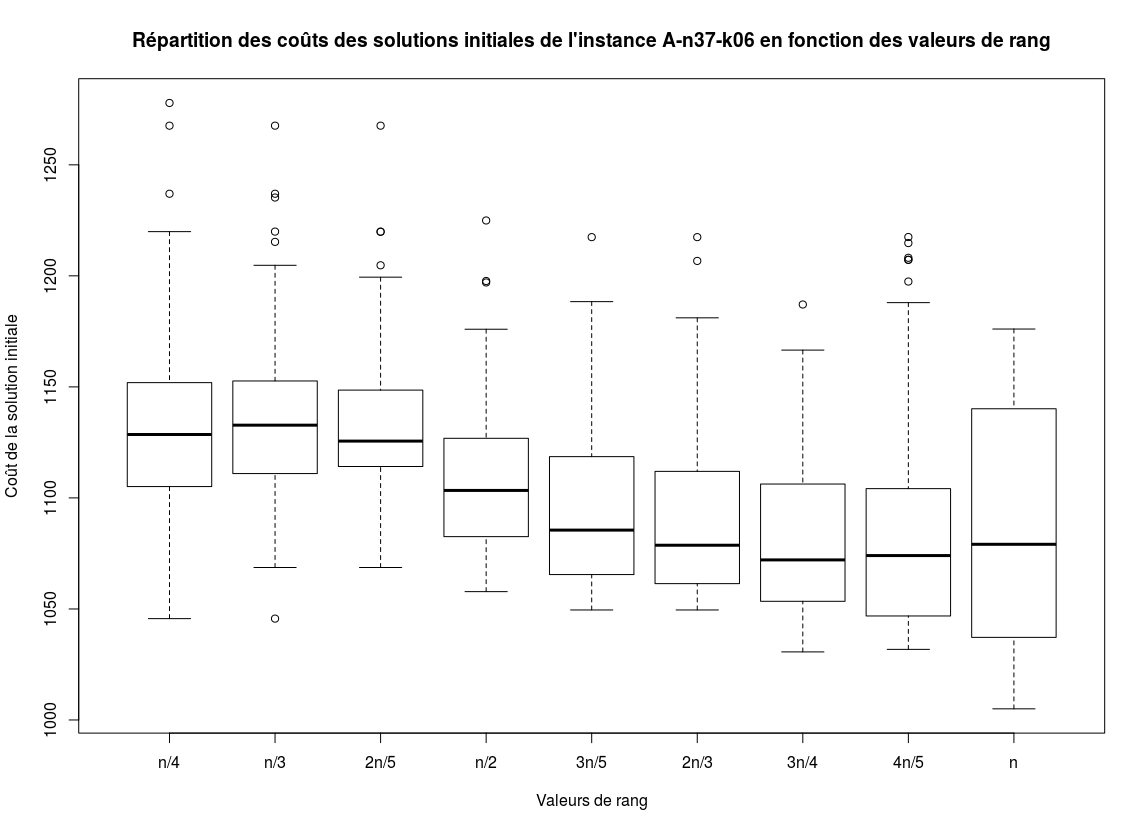
\includegraphics[scale=0.25]{InfluenceRangA3706}
        
        \caption{Influence du Rang lors de l'apprentissage sur l'instance A-n37-k06.}
        \label{InfRA3706}

    \end{minipage}
    \hfill%
    \begin{minipage}[c]{.46\linewidth}
        \centering
        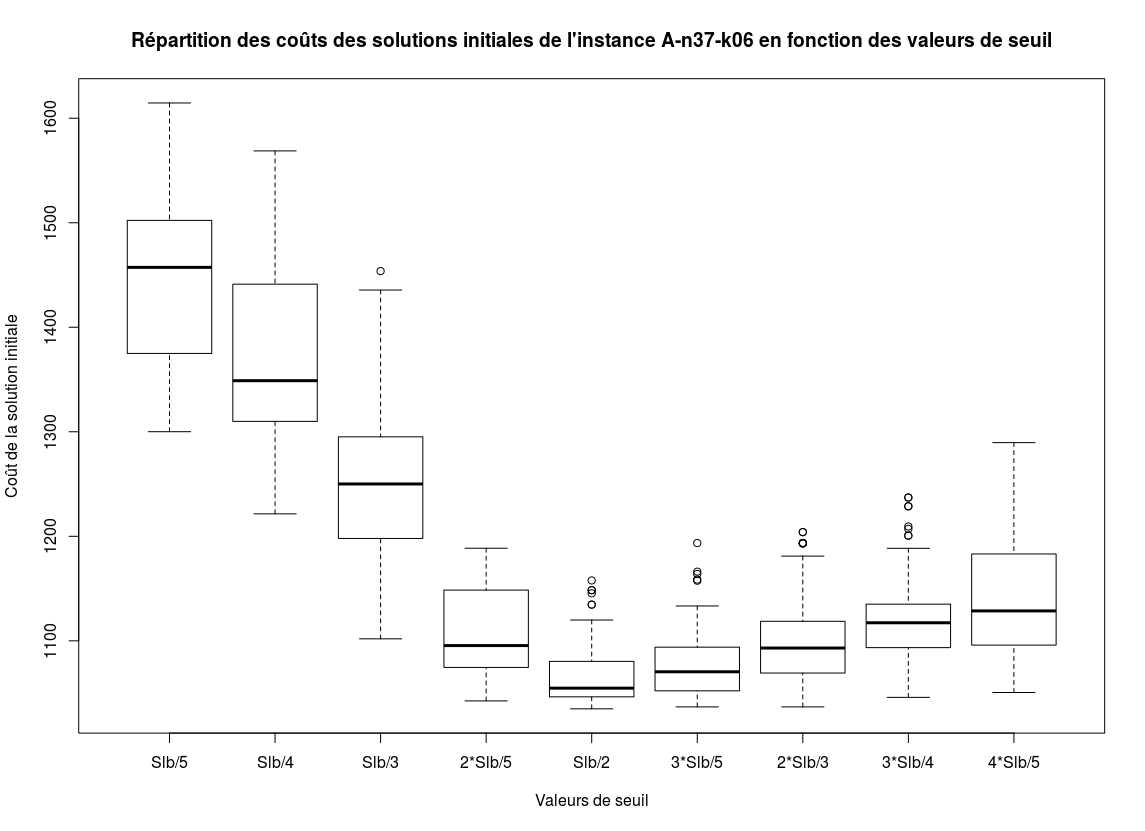
\includegraphics[scale=0.25]{InfluenceSeuilA3706}
        
        \caption{Influence du Seuil lors de l'apprentissage sur l'instance A-n37-k06.}
        \label{InfSA3706}
    \end{minipage}
    
    \begin{minipage}[c]{.46\linewidth}
        \centering
        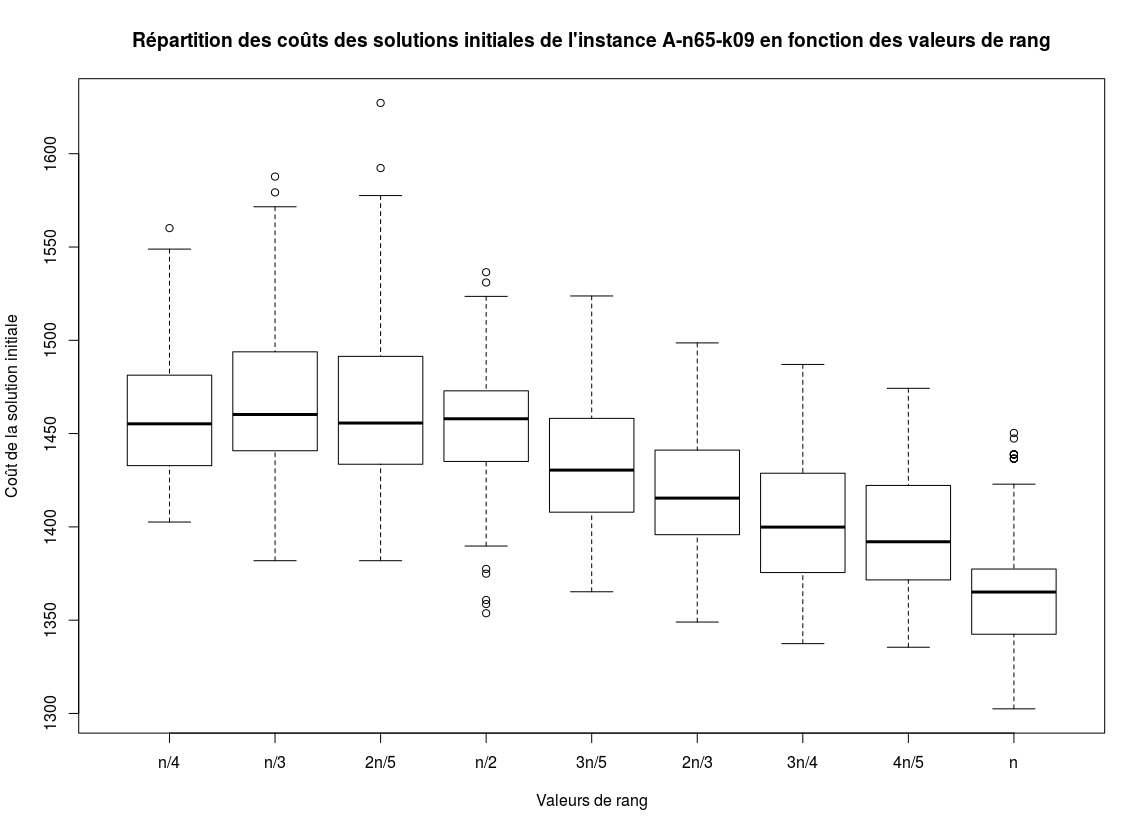
\includegraphics[scale=0.25]{InfluenceRangA6509}
        
        \caption{Influence du Rang lors de l'apprentissage sur l'instance A-n65-k09.}
        \label{InfRA6509}
    \end{minipage}
    \hfill%
    \begin{minipage}[c]{.46\linewidth}
        \centering
        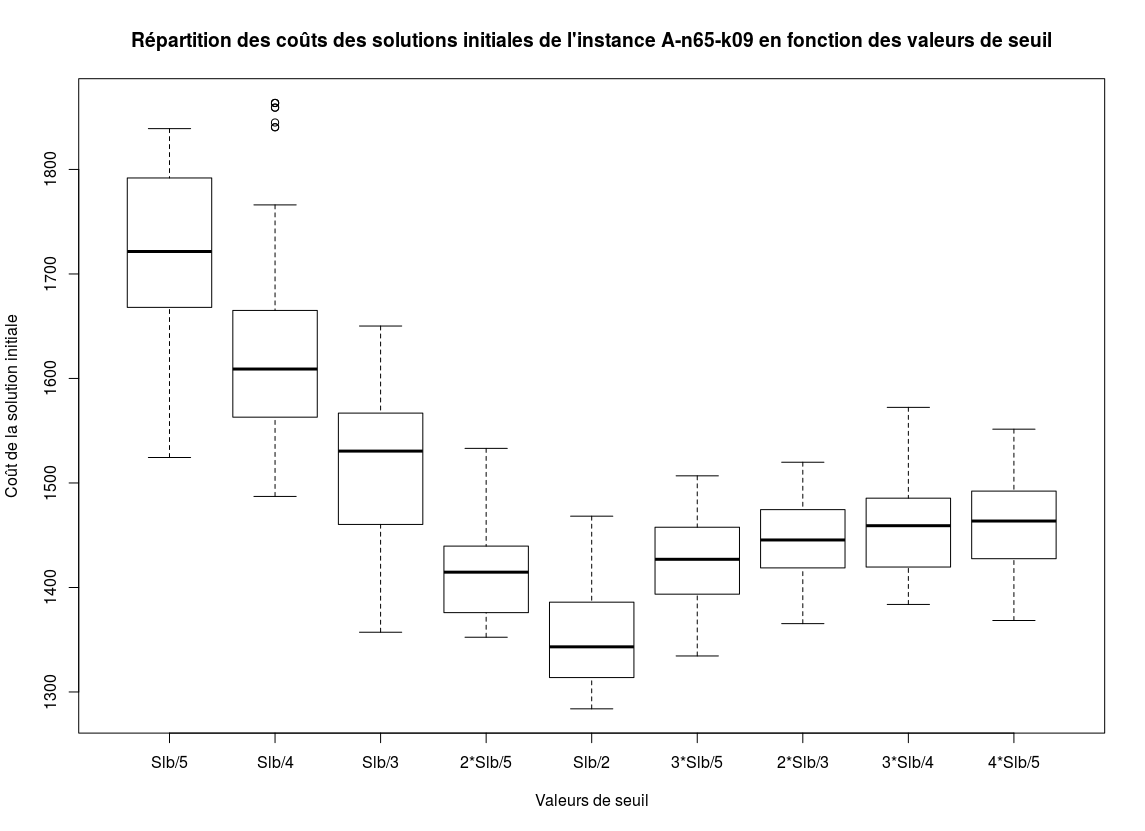
\includegraphics[scale=0.25]{InfluenceSeuilA6509}
        
        \caption{Influence du Seuil lors de l'apprentissage sur l'instance A-n65-k09.}
        \label{InfSA6509}
    \end{minipage}    
    
        \begin{minipage}[c]{.46\linewidth}
        \centering
        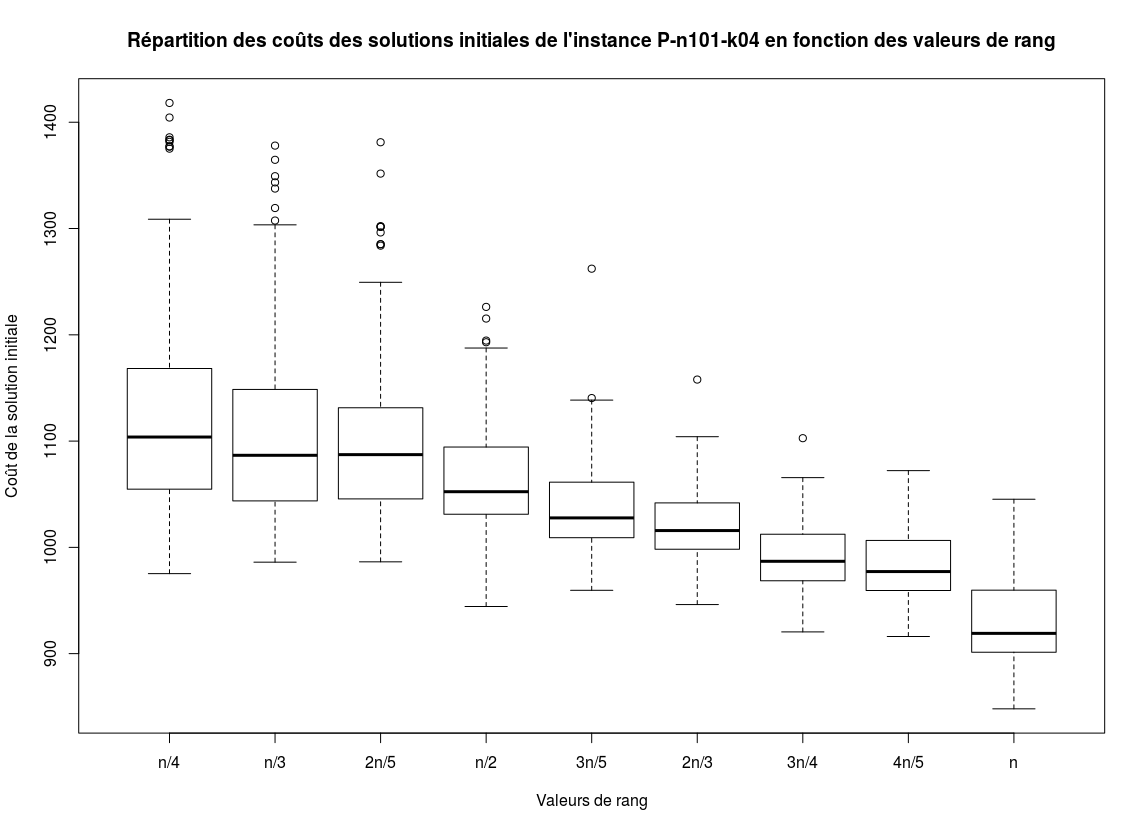
\includegraphics[scale=0.25]{InfluenceRangP10104}
        
        \caption{Influence du Rang lors de l'apprentissage sur l'instance P-n101-k04.}
        \label{InfRP10104}
    \end{minipage}
    \hfill%
    \begin{minipage}[c]{.46\linewidth}
        \centering
        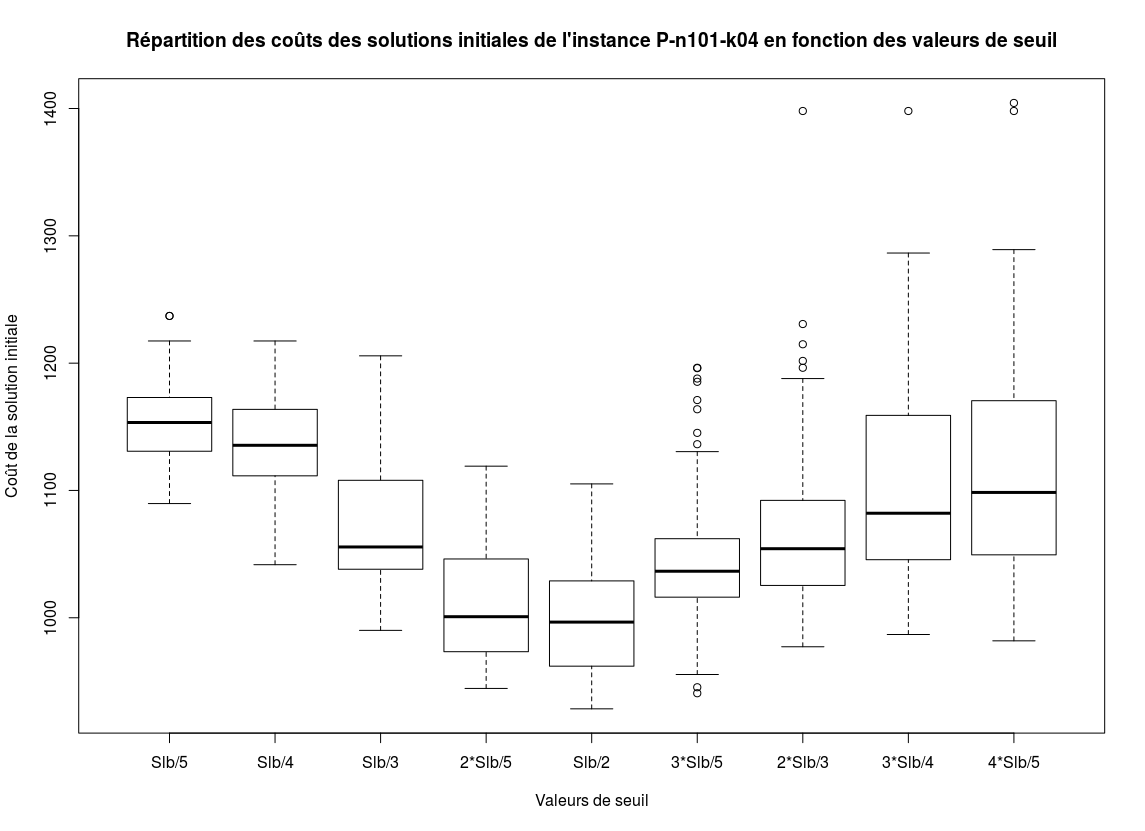
\includegraphics[scale=0.25]{InfluenceSeuilP10104}
        
        \caption{Influence du Seuil lors de l'apprentissage sur l'instance P-n101-k04.}
        \label{InfSP10104}
    \end{minipage}
\end{figure}




\section{Intégration de la connaissance} 
\label{Integration}
Cette section s'intéresse à l'intégration de connaissance dans l'algorithme d'optimisation retenu, i.e. l'algorithme~\ref{algo:HC}. 
Nous commençons par expliquer où la connaissance va être intégrée, puis nous présenterons la \emph{Learning Heuristic} créée. Enfin nous présenterons les résultats obtenus avec cette heuristique sur des instances de la littérature.

\subsection{Où intégrer la connaissance ?}
Grâce à l'extraction de connaissances nous disposons désormais d'un ensemble d'arêtes dont la plupart appartiennent à la solution optimale. 
Nous pouvons donc recréer à partir de ces arêtes des morceaux de tournées et rattacher leurs extrémités aux dépôts, comme le montre la figure~\ref{newInit}.
Cette solution temporaire, que l'on appellera \emph{Init}, peut alors être utilisée comme initialisation pour l'algorithme CW.
En effet, l'algorithme va conserver les morceaux de tournées, qui ont été fixées lors de l'apprentissage, et va fusionner ces morceaux entre eux, pour obtenir au final une nouvelle solution initiale.

Cette solution initiale pourra ensuite être utilisée dans l'algorithme d'optimisation $H_c$.

Néanmoins il faut trouver un nouveau triplet de paramètre $(\lambda^*,\mu^*,\nu^*)$ pour pouvoir appliquer CW. Nous décidons pour cela de choisir le triplet associé à la solution de coût le plus faible présente dans l'échantillon, i.e. vérifiant :
\begin{center}
$(\lambda^*,\mu^*,\nu^*) = argmin_{(\lambda,\mu,\nu) \in Echantillon} CW((\lambda,\mu,\nu))$
\end{center}

\begin{figure}[h!]
    \begin{minipage}[c]{.46\linewidth}
        \centering
        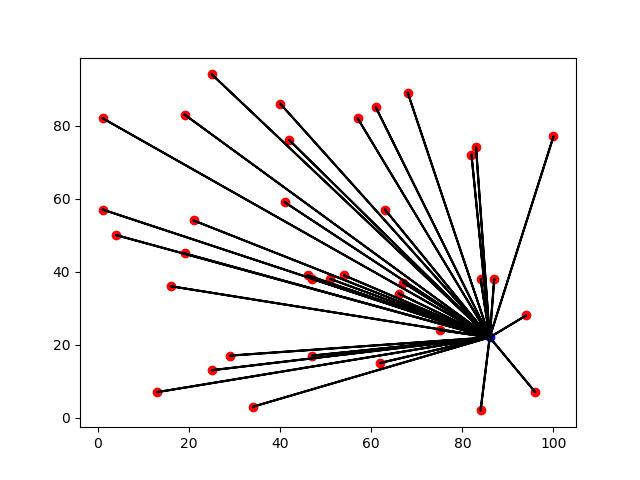
\includegraphics[scale=0.4]{CWinit.png}
        \caption{Initialisation habituelle de CW.}
    \end{minipage}
    \hfill%
    \begin{minipage}[c]{.46\linewidth}
        \centering
        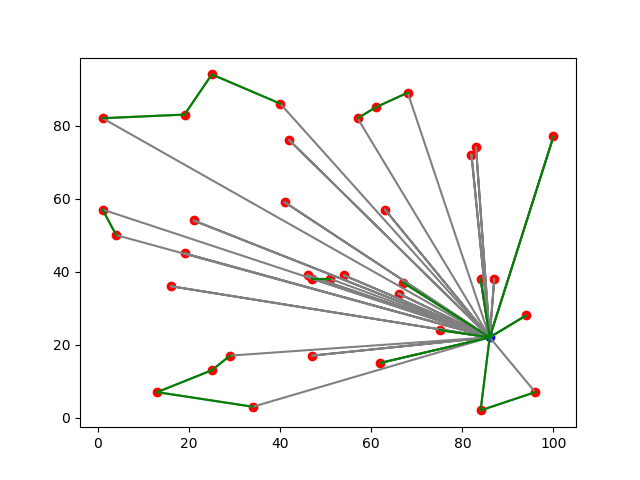
\includegraphics[scale=0.4]{learning.png}
        \caption{Initialisation de CW après apprentissage : \emph{Init}.}
        \label{newInit}
    \end{minipage}
\end{figure}

Nous disposons enfin de tous les outils nécessaires à la création de la \emph{Learning Heuristic}.

\subsection{Learning Heuristic}
La \emph{Learning Heuristic} est présenté sur l'algorithme~\ref{algo:LH}.

\begin{algorithm}
\DontPrintSemicolon % Some LaTeX compilers require you to use \dontprintsemicolon instead
\KwIn{Un ensemble de points I, les demandes des clients D}
\KwOut{Une solution au problème I}
$(\lambda^*,\mu^*,\nu^*), Init \gets Apprentissage()$\;
$newBase \gets \{\} $\;
$bestCost \gets cost(Init)$\;
\For {$i \gets 1$ \textbf{to} $NbIterations$} {
	$Sol \gets H_c(I,D,\lambda^*,\mu^*,\nu^*,Init)$\;
	$newBase \gets newBase \cup \{Sol\}$\;
	\If {$cost(Sol) < bestCost$ or $i = 0$} {
		$bestSol \gets Sol$\;
		$bestCost \gets cost(Sol)$\;
	}
	\If {$ i\%4 = 0$ and $i \neq 0$} {
		Déterminer $Init$ en apprenant de $newBase$\;
		$(\lambda^*,\mu^*,\nu^*), Init \gets Apprentissage(Init)$\;
	}
	\Else {
		Conserver $p\%$ des arêtes de $bestSol$\;
		Construire un nouvel $Init$ avec les arêtes conservées\;
		$(\lambda^*,\mu^*,\nu^*), Init \gets Apprentissage(Init)$\;
	}
}

\Return{$bestSol$}\;
\caption{{\sc LearnHeuristic} renvoie une solution d'une instance du CVRP}
\label{algo:LH}
\end{algorithm}

Cette heuristique a l'avantage de procéder à plusieurs apprentissages. 
Mis à part l'apprentissage initial qui sert à guider les premiers résultats, les solutions ensuite calculées sont stockées dans une nouvelle base d'apprentissage, utilisée pour déterminer un nouvel $Init$.
Ce dernier est utilisé pour guider un nouvel apprentissage, et la base d'apprentissage est remise à zéro. 
Répéter ces étapes permet d'affiner l'apprentissage, pour le rendre plus efficace et ainsi approcher d'autant mieux la solution optimale.


\subsection{Résultats}

\subsubsection{Comparaison avec des ensembles d'instances résolues}

La \emph{learning heuristic} précédente a été appliquée aux ensembles d'instance A, B et P (disponibles sur le site~\cite{cvrplib}.

Pour effectuer la phase d'apprentissage (décrite dans la section~\ref{extraction}), nous choisissons de prendre un échantillon de taille $50$, nous utilisons la base $Qual_{10}$, et le critère $ rang = n/2$. Nous choisissons ensuite les valeurs suivantes dans les algorithmes utilisés : $ NbIterations = 10$, $NbSol = 10$, $limitTime = 10$, $restartTime = 0.5$, $resetTime = 0.25$.

Les résultats obtenus sont disponibles sur les tableaux~\ref{TA} à~\ref{TP}, la colonne \emph{Best-Known} rappelle le coût de la meilleure solution connue pour l'instance considérée. 
Les résultats fournis sont ceux obtenus lors de l'exécution de l'algorithme considéré.
\emph{Best} renvoie la meilleure solution sur les $100$ obtenues, \emph{Mean$_{10}$} renvoie la moyenne des $10$ meilleures solutions, \emph{Gap} correspond au pourcentage de différence entre la \emph{Best} et la \emph{Best-Known}, \emph{Time} donne le temps d'exécution de l'algorithme.

\begin{table}[h!]
\caption{Résultats pour l'ensemble A}
\label{TA}
\begin{center}
\begin{tabular}{|@{}c@{}|@{}c@{}|@{}c@{}|@{}c@{}|@{}c@{}|@{}c@{}|}

\hline
 Instance & Best-Known & \multicolumn{4}{c|}{LearnHeuristic}  \\
 \hline
 & & Best & Mean$_{10}$ & Gap (\%) & Time (s) \\ 
 \hline
 A-n32-k05 & 784 & 785 & 785 & 0.13 & 179  \\
 \hline
 A-n33-k05   & 661 & 661 & 661 &0 & 235   \\
  \hline
   A-n33-k06 & 742 & 742 & 742 &0 & 160  \\
 \hline
   A-n34-k05 & 778 & 779 & 779 &0.13 & 173  \\
  \hline
   A-n36-k05 & 799 & 799 & 799 & 0 & 222  \\
 \hline
  A-n37-k05  & 669 & 670 & 671 & 0.15 & 181  \\
  \hline
  A-n37-k06 & 949 & 949 & 949 & 0 & 174 \\
 \hline
  A-n38-k05  & 730 & 730 & 736 & 0 & 196 \\
 \hline
 A-n39-k05 & 822 & 822 & 822 & 0 & 212 \\
 \hline
  A-n39-k06  & 831 & 831 & 831 & 0 & 220   \\
 \hline
   A-n44-k06 & 937 & 937 & 937 & 0 & 232   \\
  \hline
   A-n45-k06 & 944 & 953 & 954 & 0.94 & 228  \\
 \hline 
  A-n45-k07  & 1146 & 1149 & 1151 & 0.26 & 415 \\
  \hline
  A-n46-k07  & 914 & 914 & 916 &0 & 286  \\
  \hline
  A-n48-k07 & 1073 & 1073 & 1078 &0 & 442  \\
 \hline
  A-n53-k07  & 1010 & 1014 & 1017 &0.39 & 387   \\
  \hline
  A-n54-k07  & 1167 & 1172 & 1172 & 0.26 & 273  \\
  \hline
  A-n55-k09 & 1073 & 1073 & 1073 &0 & 285  \\
 \hline 
   A-n60-k09 & 1354 & 1354 & 1356 &0 & 453   \\
  \hline 
  A-n61-k09  & 1034 & 1035 & 1038 &0.09 & 386  \\
  \hline
    A-n62-k08  & 1288 & 1308  & 1310 &1.53 & 440   \\
  \hline
    A-n63-k09  & 1616 & 1627 & 1636 &0.68 & 429   \\
  \hline
    A-n63-k10  & 1314 & 1320 &1320 &0.45 & 458   \\
  \hline
    A-n64-k09  & 1401 & 1416 & 1419 &1.06 & 463   \\
  \hline
    A-n65-k09  & 1174 & 1176 & 1180 &0.17 & 447   \\
  \hline
    A-n69-k09  & 1159 & 1164 & 1167 & 0.43 & 317   \\
  \hline
    A-n80-k10  & 1763 & 1767 & 1773 & 0.23 & 575   \\
  \hline
\end{tabular}
\end{center}
\end{table}

\begin{table}[h!]
\caption{Résultats pour l'ensemble B}
\label{TB}
\begin{center}
\begin{tabular}{|@{}c@{}|@{}c@{}|@{}c@{}|@{}c@{}|@{}c@{}|@{}c@{}|}

\hline
 Instance & Best-Known & \multicolumn{4}{c|}{LearnHeuristic}  \\
 \hline
 & & Best & Mean$_{10}$ & Gap (\%) & Time (s) \\ 
 \hline
 B-n31-k05 & 672 & 672 & 672 & 0 & 161 \\
 \hline
 B-n34-k05   & 788 & 788 & 788 &0 & 192  \\
  \hline
   B-n35-k05 & 955 & 955 & 957 &0 & 169  \\
 \hline
   B-n38-k06 & 805 & 806 & 806 &0.12 & 238  \\
  \hline
   B-n39-k05 & 549 & 550 & 550 & 0.18 & 267  \\
 \hline
  B-n41-k06  & 829 & 831 & 831 & 0.24 & 206  \\
  \hline
  B-n43-k06 & 742 & 742 & 742 & 0 & 302 \\
 \hline
  B-n44-k07  & 909 & 910 & 910 & 0.11 & 203 \\
 \hline
 B-n45-k05 & 751 & 751 & 751 & 0 & 207 \\
 \hline
   B-n50-k07 & 741 & 741 & 741 & 0 & 299   \\
  \hline
   B-n50-k08 & 1312 & 1320 & 1327 & 0.61 & 255  \\
  \hline
  B-n52-k07  & 747 & 747 & 748 &0 & 365  \\
  \hline
  B-n56-k07 & 707 & 710 & 710 & 0.42 & 297  \\
 \hline
  B-n57-k09  & 1598 & 1599 & 1601 &0.06 & 306   \\
  \hline
  B-n63-k10  & 1496 & 1537 & 1540 & 2.66 & 338   \\
  \hline
  B-n64-k09 & 861 & 866 & 870 & 0.58 & 303 \\
 \hline 
   B-n66-k09 & 1316 & 1321 & 1324 &0.38 & 385   \\
  \hline 
  B-n67-k10  & 1032 & 1040 & 1041 & 0.77 & 425  \\
  \hline
    B-n68-k09  & 1272 & 1289 & 1290 &1.32 & 452   \\
  \hline
    B-n78-k10  & 1221 & 1231 & 1238 & 0.57 & 526 \\
  \hline
\end{tabular}
\end{center}
\end{table}

\begin{table}[h!]
\caption{Résultats pour l'ensemble P}
\label{TP}
\begin{center}
\begin{tabular}{|@{}c@{}|@{}c@{}|@{}c@{}|@{}c@{}|@{}c@{}|@{}c@{}|}

\hline
 Instance & Best-Known & \multicolumn{4}{c|}{LearnHeuristic}  \\
 \hline
 & & Best & Mean$_{10}$ & Gap (\%) & Time (s) \\ 
 \hline
 P-n016-k08 & 450 & 450 & 450 & 0 & 52  \\
 \hline
 P-n019-k02   & 212 & 212 & 215 & 0 & 65   \\
  \hline
   P-n020-k02 & 216 & 216 & 216 &0 & 72  \\
 \hline
   P-n021-k02 & 211 & 211 & 211 &0 & 83  \\
  \hline
   P-n022-k02 & 216 & 216 & 216 & 0 & 101  \\
 \hline
  P-n023-k08  & 529 & 529 & 530 & 0 & 82 \\
  \hline
  P-n040-k05 & 458 & 458 & 458 & 0 & 171 \\
 \hline
  P-n045-k05  & 510 & 510 & 510 & 0 & 260 \\
 \hline
 P-n050-k07 & 554 & 554 & 555 & 0 & 342 \\
 \hline
  P-n050-k08  & 631 & 631 & 633 & 0 & 333   \\
 \hline
   P-n050-k10 & 696 & 699 & 701 & 0.43 & 368   \\
  \hline
   P-n051-k10 & 741 & 742 & 747 & 0.13 & 401  \\
 \hline 
  P-n055-k07  & 568 & 568 & 572& 0 & 541  \\
  \hline
  P-n055-k10  & 694 & 694 & 699 &0 & 469  \\
  \hline
  P-n060-k10 & 744 & 750 & 751 & 0.8 & 339  \\
 \hline
   P-n060-k15  & 968 & 979 & 979 &1.12 & 258   \\
  \hline
  P-n065-k10  & 792 & 792 & 792 & 0 & 398   \\
  \hline
  P-n070-k10 & 827 & 833 & 838 & 0.72 & 373    \\
  \hline
  P-n076-k04 & 593 & 596 &600 & 0.50 & 436 \\
 \hline 
   P-n076-k05 & 627 & 631 & 638 &0.63 & 424   \\
  \hline 
  P-n101-k04  & 681 & 686 & 687 & 0.73 & 573  \\
  \hline
\end{tabular}
\end{center}
\end{table}

La plupart des solutions obtenus avec l'algorithme \lstinline|LearnHeuristic| sont très proches des solutions optimales, comme le montrent les résultats moyens présentés dans le tableau~\ref{Synth}. 
Il est possible qu'en changeant la méthode d'apprentissage, ou le temps disponible dans $H_c$, on obtienne de meilleurs résultats. Néanmoins les paramètres choisis, permettent d'avoir un algorithme à la fois rapide et efficace. 

\begin{table}[h!]
\caption{Synthèse des résultats pour les ensembles A, B et P}
\label{Synth}
\begin{center}
\begin{tabular}{|c|c|c|c|}

\hline
 Instances & Size & Gap (\%) & Time (s)  \\
 \hline
 Group A & 27 & 0.26 & 8468  \\
 \hline
 Group B & 20  & 0.40 & 5816   \\
  \hline
  Group P & 21 & 0.24 & 6141   \\
 \hline

\end{tabular}
\end{center}
\end{table}

\subsubsection{Résultats obtenus sur les problèmes plus difficiles}

Dans cette section sont présentés les résultats obtenus sur les ensembles \emph{Golden} et \emph{Uchoa}.

\section*{Conclusion}
A travers cet article, nous avons vu comment créer une \emph{learning heuristic} donnant de très bons résultats sur les instances classiques du CVRP.
L'avantage aussi de cet algorithme est qu'il vient compléter un algorithme d'optimisation facilement adaptable à d'autres problèmes de tournées de véhicules (comme le problème multi-dépôts~\cite{Sorensen_2017}).
 
Toutefois cette méta-heuristique reste longue à exécuter, il pourrait donc être intéressant de voir si une autre condition d'arrêt à $H_c$ donne d'aussi bons résultats, avec un meilleur temps d'exécution.


\section*{Remerciements}
Je tiens à remercier l'équipe ORKAD, du centre CRIStAL de Lille, qui m'a aidé à réaliser ce projet. Je remercie plus particulièrement Laetitia Jourdan (laetitia.jourdan@univ-lille.fr), Marie-Éléonore Kessaci (me.kessaci@univ-lille.fr), membres de l'équipe ORKAD, ainsi que Diego Cattaruzza (diego.cattaruzza@ec-lille.fr) membre de l'équipe INOCS, qui m'ont encadré pendant la durée de ce projet.



\bibliographystyle{plain}
\bibliography{biblio}

\end{document}